\documentclass{beamer}
\mode<presentation>
{
  \usetheme{Darmstadt}
  \definecolor{BYUBlue}{RGB}{00,22,55}
  \definecolor{BYUTan}{RGB}{232,211,175}
  \usecolortheme[named=BYUBlue]{structure}
  \setbeamercolor*{palette primary}{use=structure,fg=BYUBlue,bg=lightgray}
  \setbeamercolor*{palette quaternary}{fg=white,bg=lightgray!0!BYUBlue}
  \setbeamercolor{frametitle}{fg=BYUBlue,bg=BYUBlue!10}
  \setbeamertemplate{items}[circle]
  \setbeamertemplate{blocks}[rounded][shadow=True]
  \setbeamertemplate{navigations symbols}{circle}
}

\usepackage{graphics}
\usepackage[english]{babel}
\usepackage[utf8]{inputenc}
\usepackage{times}
\usepackage{forest}
\usepackage{subfigure}
\usepackage{caption}
\captionsetup{labelformat=empty}% redefines the caption setup of the figures environment in the beamer class.
\usepackage[T1]{fontenc}
\usepackage{array}
\usepackage{amsmath,amssymb}
\usepackage{booktabs}
\usepackage{colortbl}
\usepackage{array}
\usepackage{threeparttable}
\usepackage{multirow}
\usepackage{amsthm}
\usepackage{float,graphicx,color}
\usepackage{graphics}
\usepackage{multicol}
\usepackage{natbib}
\usepackage{color}
\usepackage{hyperref}
\hypersetup{colorlinks, urlcolor=blue}
\usepackage{threeparttable}
% \usepackage[format=hang,font=normalsize,labelfont=bf]{caption}
% \usepackage{subcaption}
\usepackage{delarray}
\usepackage{amssymb}
\usepackage{setspace}
\usepackage{placeins}
\usepackage{multirow}
\usepackage{mathtools}
\usepackage{animate}
\usepackage{bm}
\usepackage{amsmath,bm}
\usepackage{amssymb}
\usepackage{amsthm}
\newtheorem*{thm}{Theorem}
\theoremstyle{definition}
\newtheorem*{defn}{Definition}
\newcommand\ve{\varepsilon}
\newcommand\norm[1]{\left\lVert#1\right\rVert}
\DeclareMathOperator*{\argmin}{argmin}

% Python code blocks --------------------------------------
\usepackage{pythonhighlight}
\usepackage{tcolorbox}
\definecolor{codegreen}{rgb}{0,0.6,0}
\definecolor{codegray}{rgb}{0.5,0.5,0.5}
\definecolor{codepurple}{rgb}{0.58,0,0.82}
\definecolor{backcolour}{rgb}{0.95,0.95,0.92}

\lstdefinestyle{mystyle}{
    backgroundcolor=\color{backcolour},
    commentstyle=\color{codegreen},
    keywordstyle=\color{magenta},
    numberstyle=\tiny\color{codegray},
    stringstyle=\color{codepurple},
    basicstyle=\ttfamily\footnotesize,
    breakatwhitespace=false,
    breaklines=true,
    captionpos=b,
    keepspaces=true,
    numbers=left,
    numbersep=5pt,
    showspaces=false,
    showstringspaces=false,
    showtabs=false,
    tabsize=2
}

\lstset{style=mystyle}

\title[OG-PHL]{OG-PHL: Current Calibration and Data Sources}

\author[DeBacker and Evans]{\textbf{Jason DeBacker} \inst{1} \and \textbf{Richard W. Evans} \inst{2}}
\institute[shortinst]{\inst{1} University of South Carolina, Department of Economics \and
\inst{2} Abundance Institute, Open Research Group, Inc.}

\date[Short Occasion]{\textbf{January 15, 2026} \\ United Nations, Philippines}


\begin{document}

\begin{frame}
  \titlepage
\end{frame}


\section{Overview}

\begin{frame}
  \frametitle{OG-PHL}

  \begin{figure}[htb]\centering
    
\includegraphics[height=0.6\textheight]{./images/OG-PHL_logo.png}
  \end{figure}

  \begin{itemize}
    \item OG-PHL is a calibration of the OG-Core model.
  \end{itemize}
\end{frame}

\begin{frame}
  \frametitle{OG-PHL: A Calibration}
  What it means for OG-PHL to be a ``calibration'' of OG-Core...
  \begin{itemize}
    \item OG-Core has all the underlying theory (e.g., different households, an arbitrary number of production sectors)
    \item But the parameters of the model are set to represent the Philippines economy
    \item E.g.,
      \begin{itemize}
        \item The model matches Philippines' gini coefficient for the distribution of income
        \item The size of production sectors represent the relative size in the Philippines economy
        \item Policy parameters are set to represent Philippines' tax system
      \end{itemize}
  \end{itemize}
  NOTE: Any of these parameters can be changed to represent a counter factual Philippines...
\end{frame}

\begin{frame}
  \frametitle{Model Dimensions}
  \begin{itemize}
    \item OG-Core allows for arbitrary sizes in the various model dimensions.  In OG-PHL, the defaults are:
      \begin{itemize}
          \item Number of labor skill groups, \textcolor{blue}{$J$: 7}
            \begin{itemize}
              \item Representing the 0-25\%, 25-50\%, 50-70\%, 70-80\%, 80-90\%, 90-99\%, Top 1\%
            \end{itemize}
          \item Age at which economically active, \textcolor{blue}{$E$: 20}
          \item Number of periods representing ages $E$ to 100, \textcolor{blue}{$S$: 80}
            \begin{itemize}
              \item With this, a model period represents one year
            \end{itemize}
          \item Number of model periods until assume reach steady-state, \textcolor{blue}{$T$: $4 \times S = 320$}
            \begin{itemize}
              \item Note, it's helpful to make $T$ a bit larger than you think it needs to be since you need the economy to settle down before this point, but only computational cost if set it too high
            \end{itemize}
          \item  Number of consumption goods, \textcolor{blue}{$I$: 1 (5)}
          \item  Number of production industries, \textcolor{blue}{$M$: 1 (7)}
      \end{itemize}
  \end{itemize}
\end{frame}

\begin{frame}
  \frametitle{OG-PHL Calibration}
  \begin{itemize}
    \item The following parameters have been calibrated specifically to Philippines:
      \begin{itemize}
          \item Demographics
          \item Lifetime earnings processes for heterogeneous households
          \item Firm production functions (labor share of output)
          \item Household consumption parameters (expenditure shares on differentiated goods)
          \item Input-output mapping between firm output and consumption categories
          \item Macro parameters (long run growth rate, gov't interest rate haircut)
          \item Remittances
      \end{itemize}
  \end{itemize}
\end{frame}

\begin{frame}
  \frametitle{OG-PHL Calibration}
  \begin{itemize}
    \item Other parameters such as:
      \begin{itemize}
          \item Household preference parameters
          \item Elasticity of substitution between capital and labor
      \end{itemize}
    \item Are set to standard values used in the literature, due to a lack of research (to our knowledge) on these parameters in the Philippines context
  \end{itemize}
\ \\
  Full documentation of the OG-PHL calibration: \href{https://EAPD-DRB.github.io/OG-PHL/}{https://EAPD-DRB.github.io/OG-PHL/}
\end{frame}

\section{Demographics}
\begin{frame}
\frametitle{OG-PHL Demographics}
  \begin{itemize}
      \item Demographic parameters include:
          \begin{itemize}
              \item Fertility rates by age
              \item Mortality rates age
              \item Age distribution of the population in an initial period
              \item \emph{Not} immigration (to ensure things add up, immigration computed as a residual)
          \end{itemize}
      \item The \href{https://population.un.org/wpp/}{UN World Population Prospects data} provide all of these for most countries from present with forecasts through 2100!
  \end{itemize}
\end{frame}

\begin{frame}{Population Dynamics}
    The population evolves according to the following laws of motion, where $\omega_{s,t}$ are the number of age $s$ households at time $t$:
    \begin{equation*}
      \begin{split}
        \omega_{1,t+1} &= (1 - \rho_0)\sum_{s=1}^{E+S} f_s\omega_{s,t} + i_1\omega_{1,t}\quad\forall t \\
        \omega_{s+1,t+1} &= (1 - \rho_s)\omega_{s,t} + i_{s+1}\omega_{s+1,t}\quad\forall t\quad\text{and}\quad 1\leq s \leq E+S-1
      \end{split}
    \end{equation*}
    \begin{itemize}
        \item The age-specific fertility rates, $f_s$, mortality rates, $\rho_s$, and immigration rates, $i_s$ affect the distribution each period
        \item Given that these rates are constant, the population distribution will converge to a steady-state distribution
    \end{itemize}
\end{frame}

    \begin{frame}{Data: Demographics}
      \begin{itemize}
        \item Demographics from the \href{https://population.un.org/wpp/}{UN Population Prospects} database
        \begin{itemize}
          \item Fertility, mortality, and population by age
          \item Historical and projected data
        \end{itemize}
      \end{itemize}
    \end{frame}


\begin{frame}
\frametitle{Philippines: Fertility and Mortality}
 \begin{figure}[ht]
      \begin{minipage}[b]{0.45\linewidth}
          \centering
          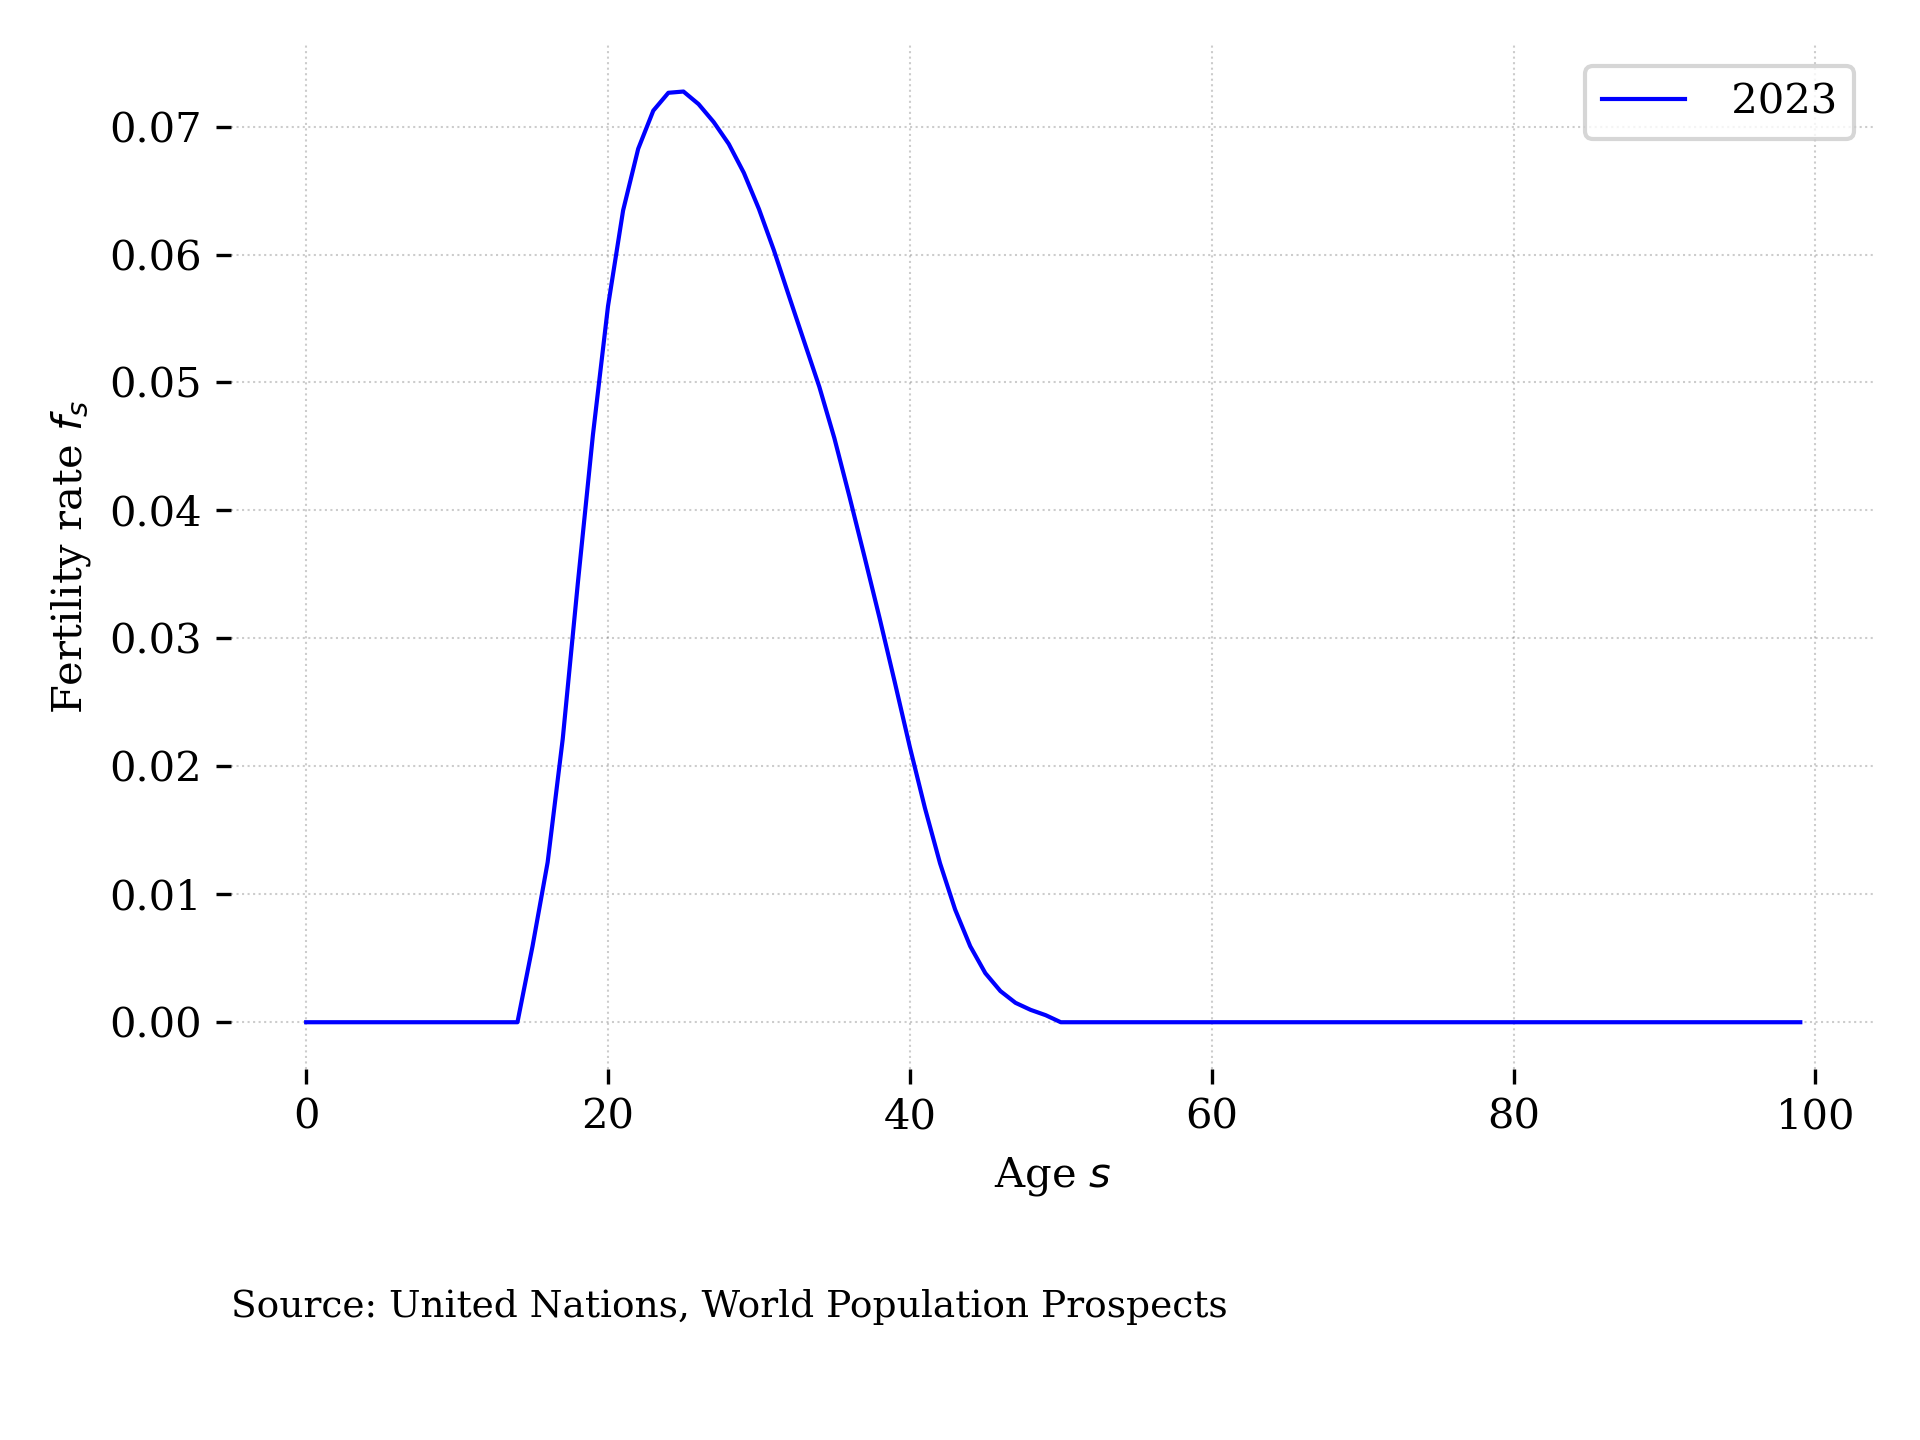
\includegraphics[width=\textwidth]{./images/fert_rates.png}
          \caption{Fertility Rates}
          \label{fig:fertility}
      \end{minipage}
      \hspace{0.5cm}
      \begin{minipage}[b]{0.45\linewidth}
          \centering
          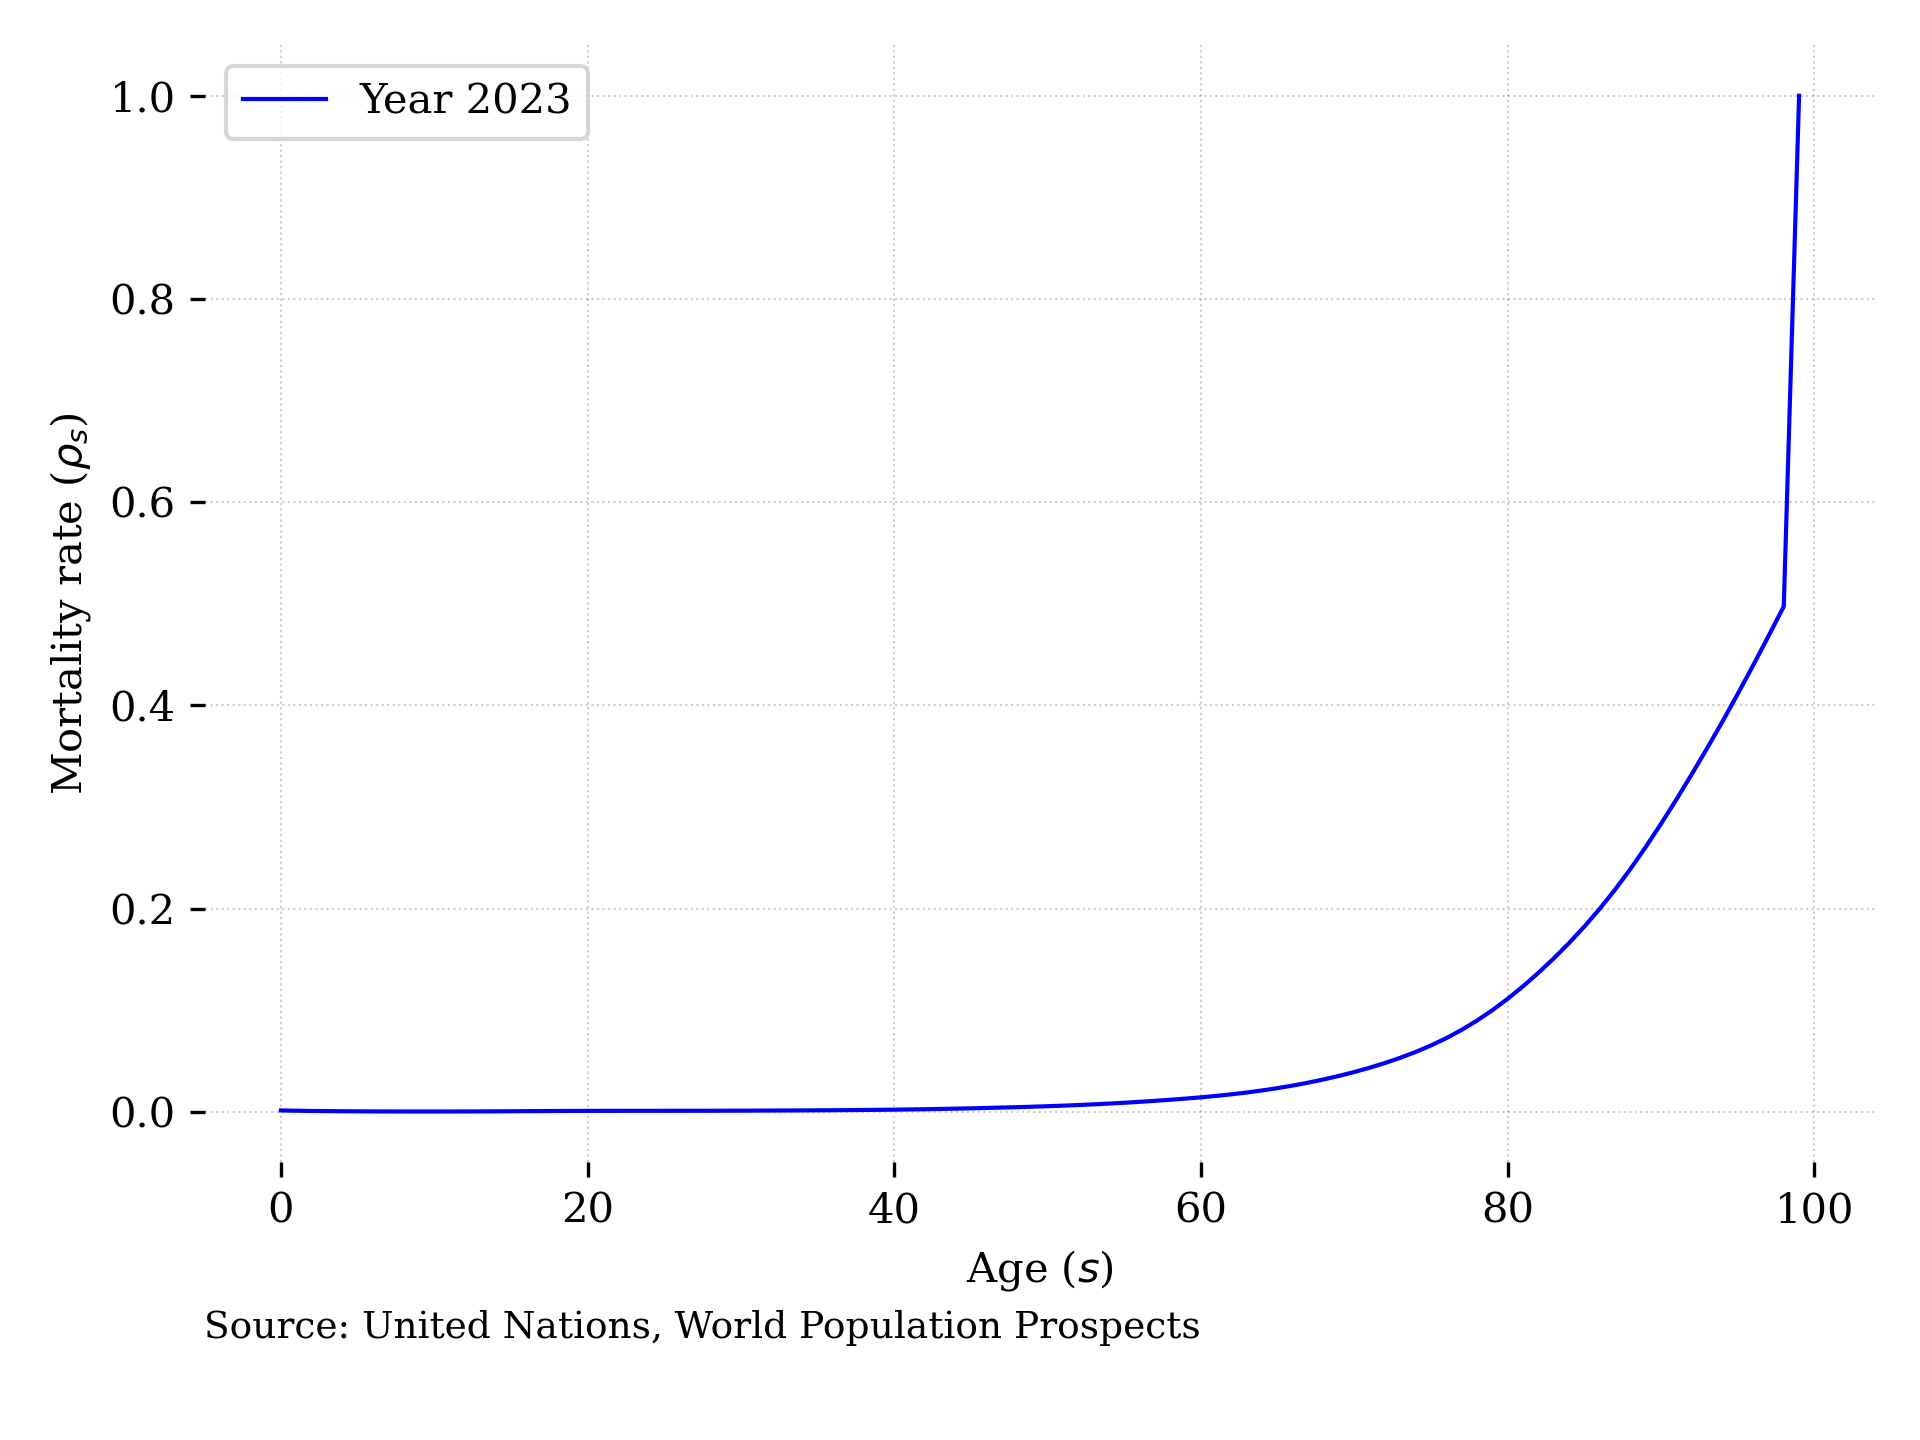
\includegraphics[width=\textwidth]{./images/mort_rates.png}
          \caption{Mortality Rates}
          \label{fig:mortality}
      \end{minipage}
  \end{figure}
 \end{frame}


\begin{frame}
\frametitle{Philippines: Demographics, immigration rates}
  \begin{figure}[htb]\centering
  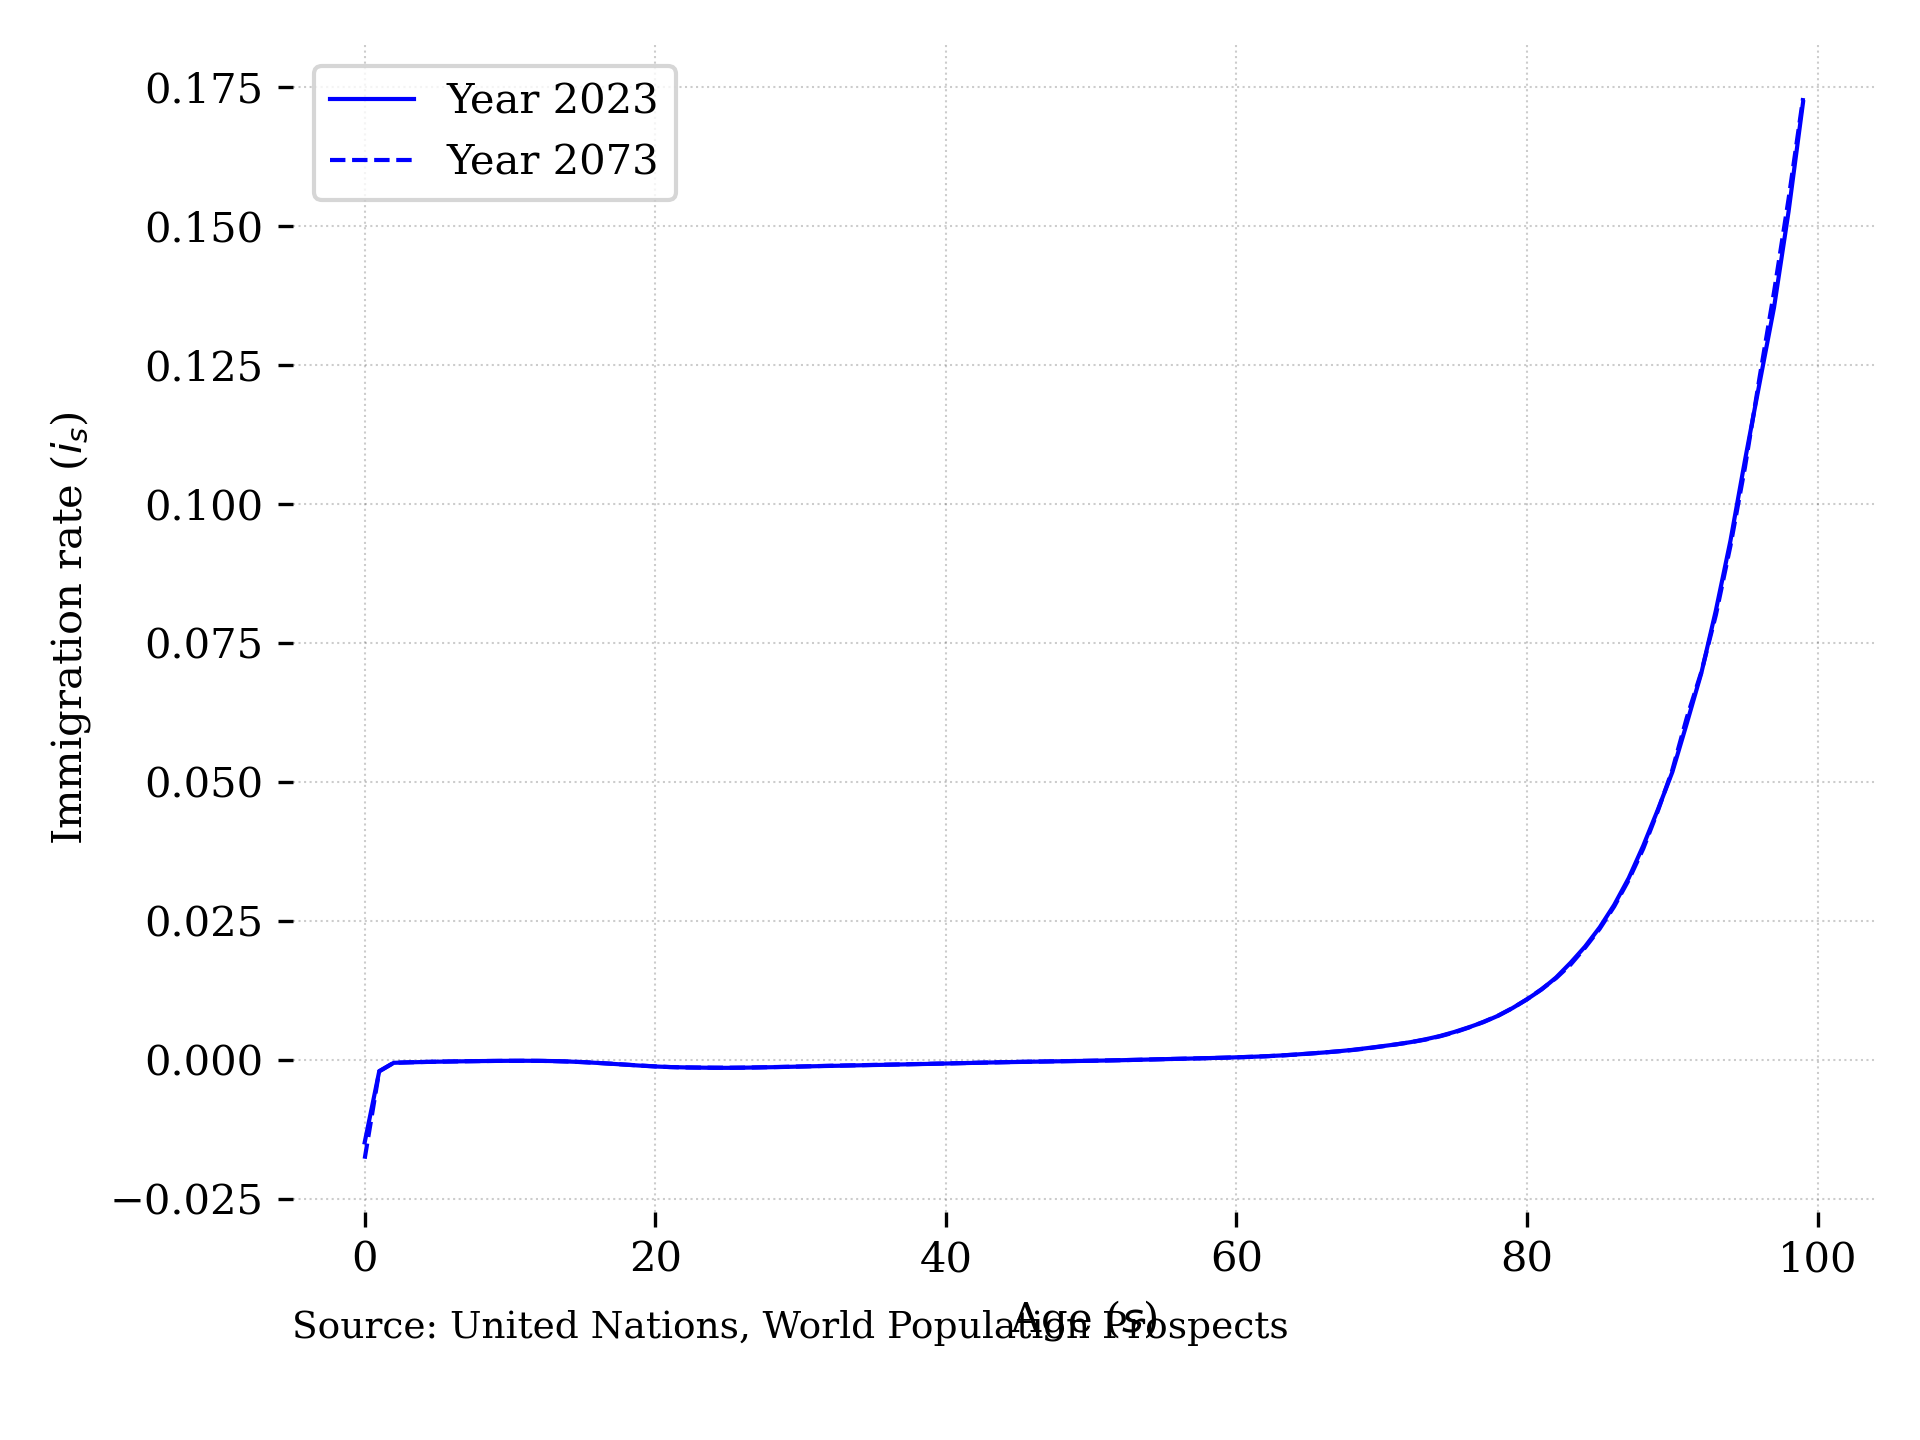
\includegraphics[height=0.8\textheight]{./images/imm_rates.png}
  \end{figure}
\end{frame}

\begin{frame}
\frametitle{Philippines: Demographics, pop. distribution}
  \begin{figure}[htb]\centering
  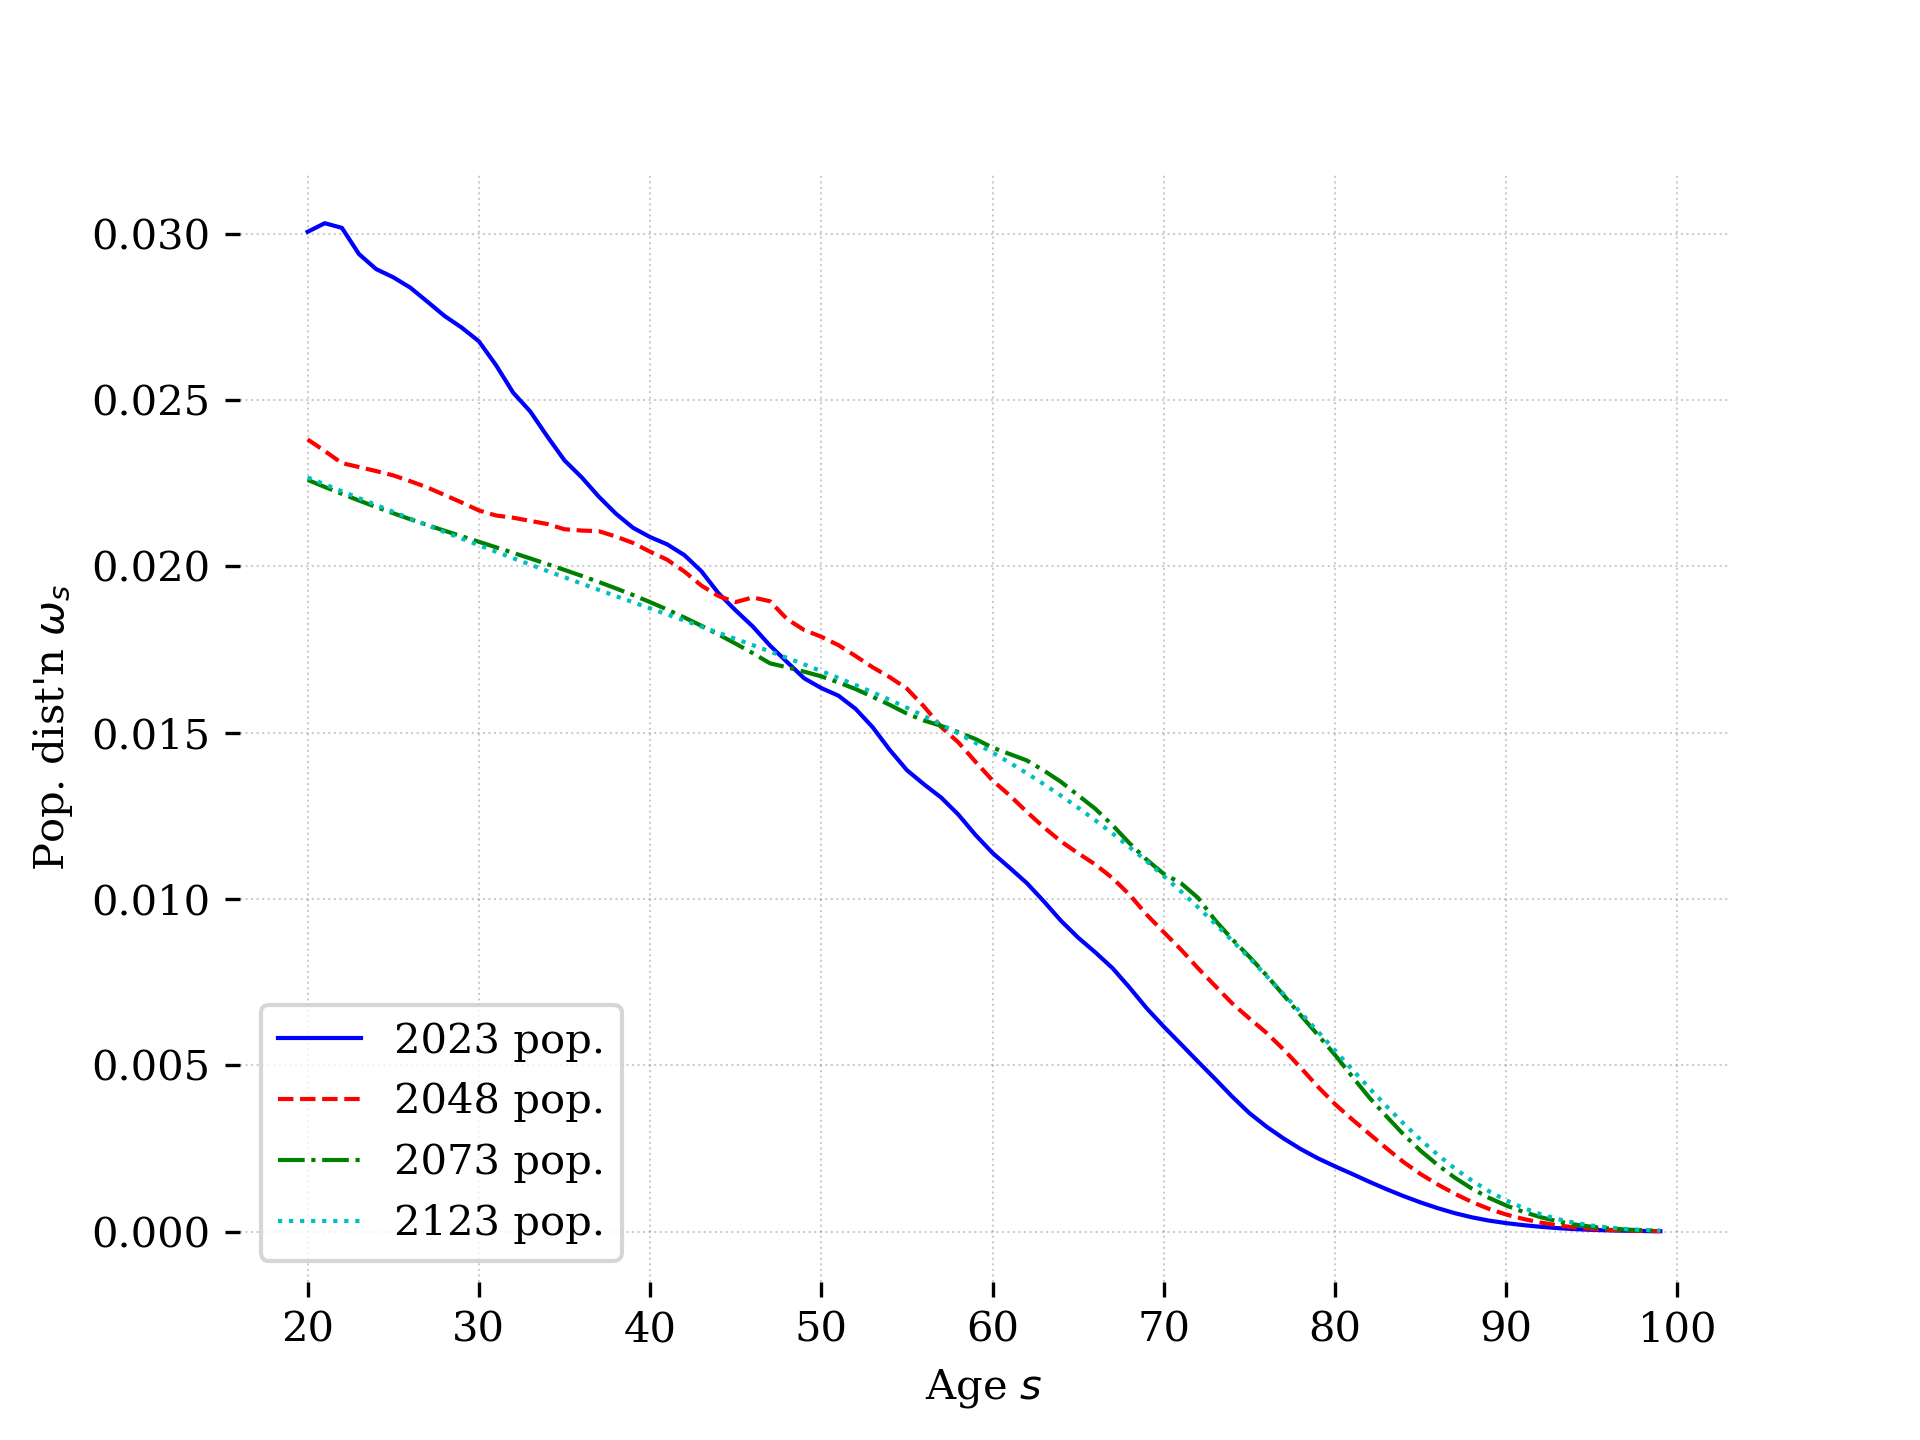
\includegraphics[height=0.8\textheight]{./images/pop_distribution.png}
  \end{figure}
\end{frame}

\begin{frame}
\frametitle{Compare to India: Demographics, pop. distribution}
  \begin{figure}[htb]\centering
  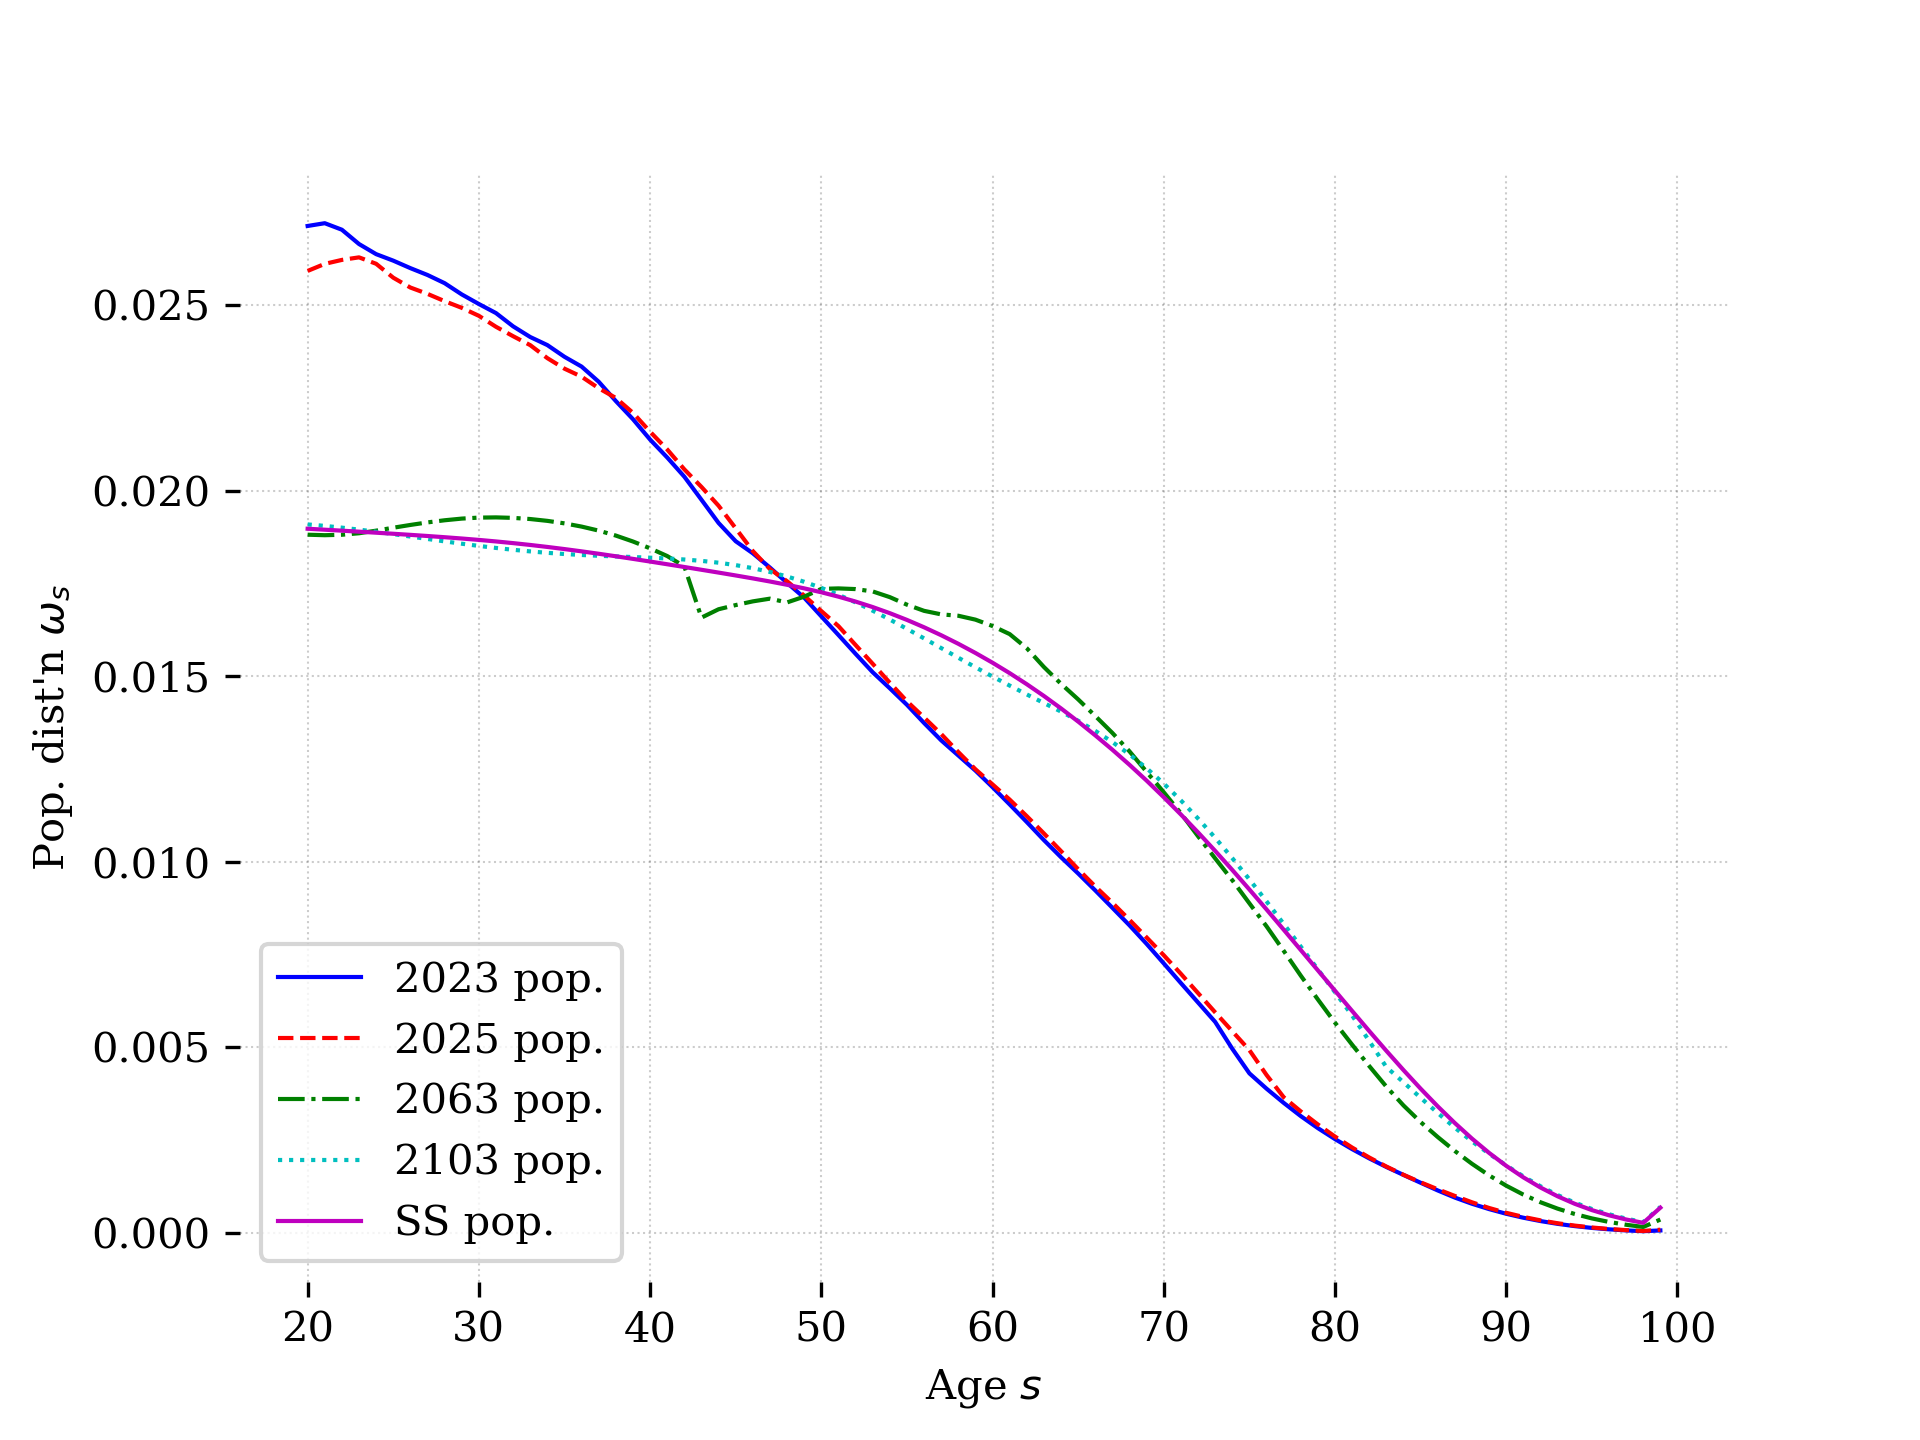
\includegraphics[height=0.8\textheight]{./images/IND_pop_distribution.png}
  \end{figure}
\end{frame}

\begin{frame}
\frametitle{Compare to USA: Demographics, pop. distribution}
  \begin{figure}[htb]\centering
  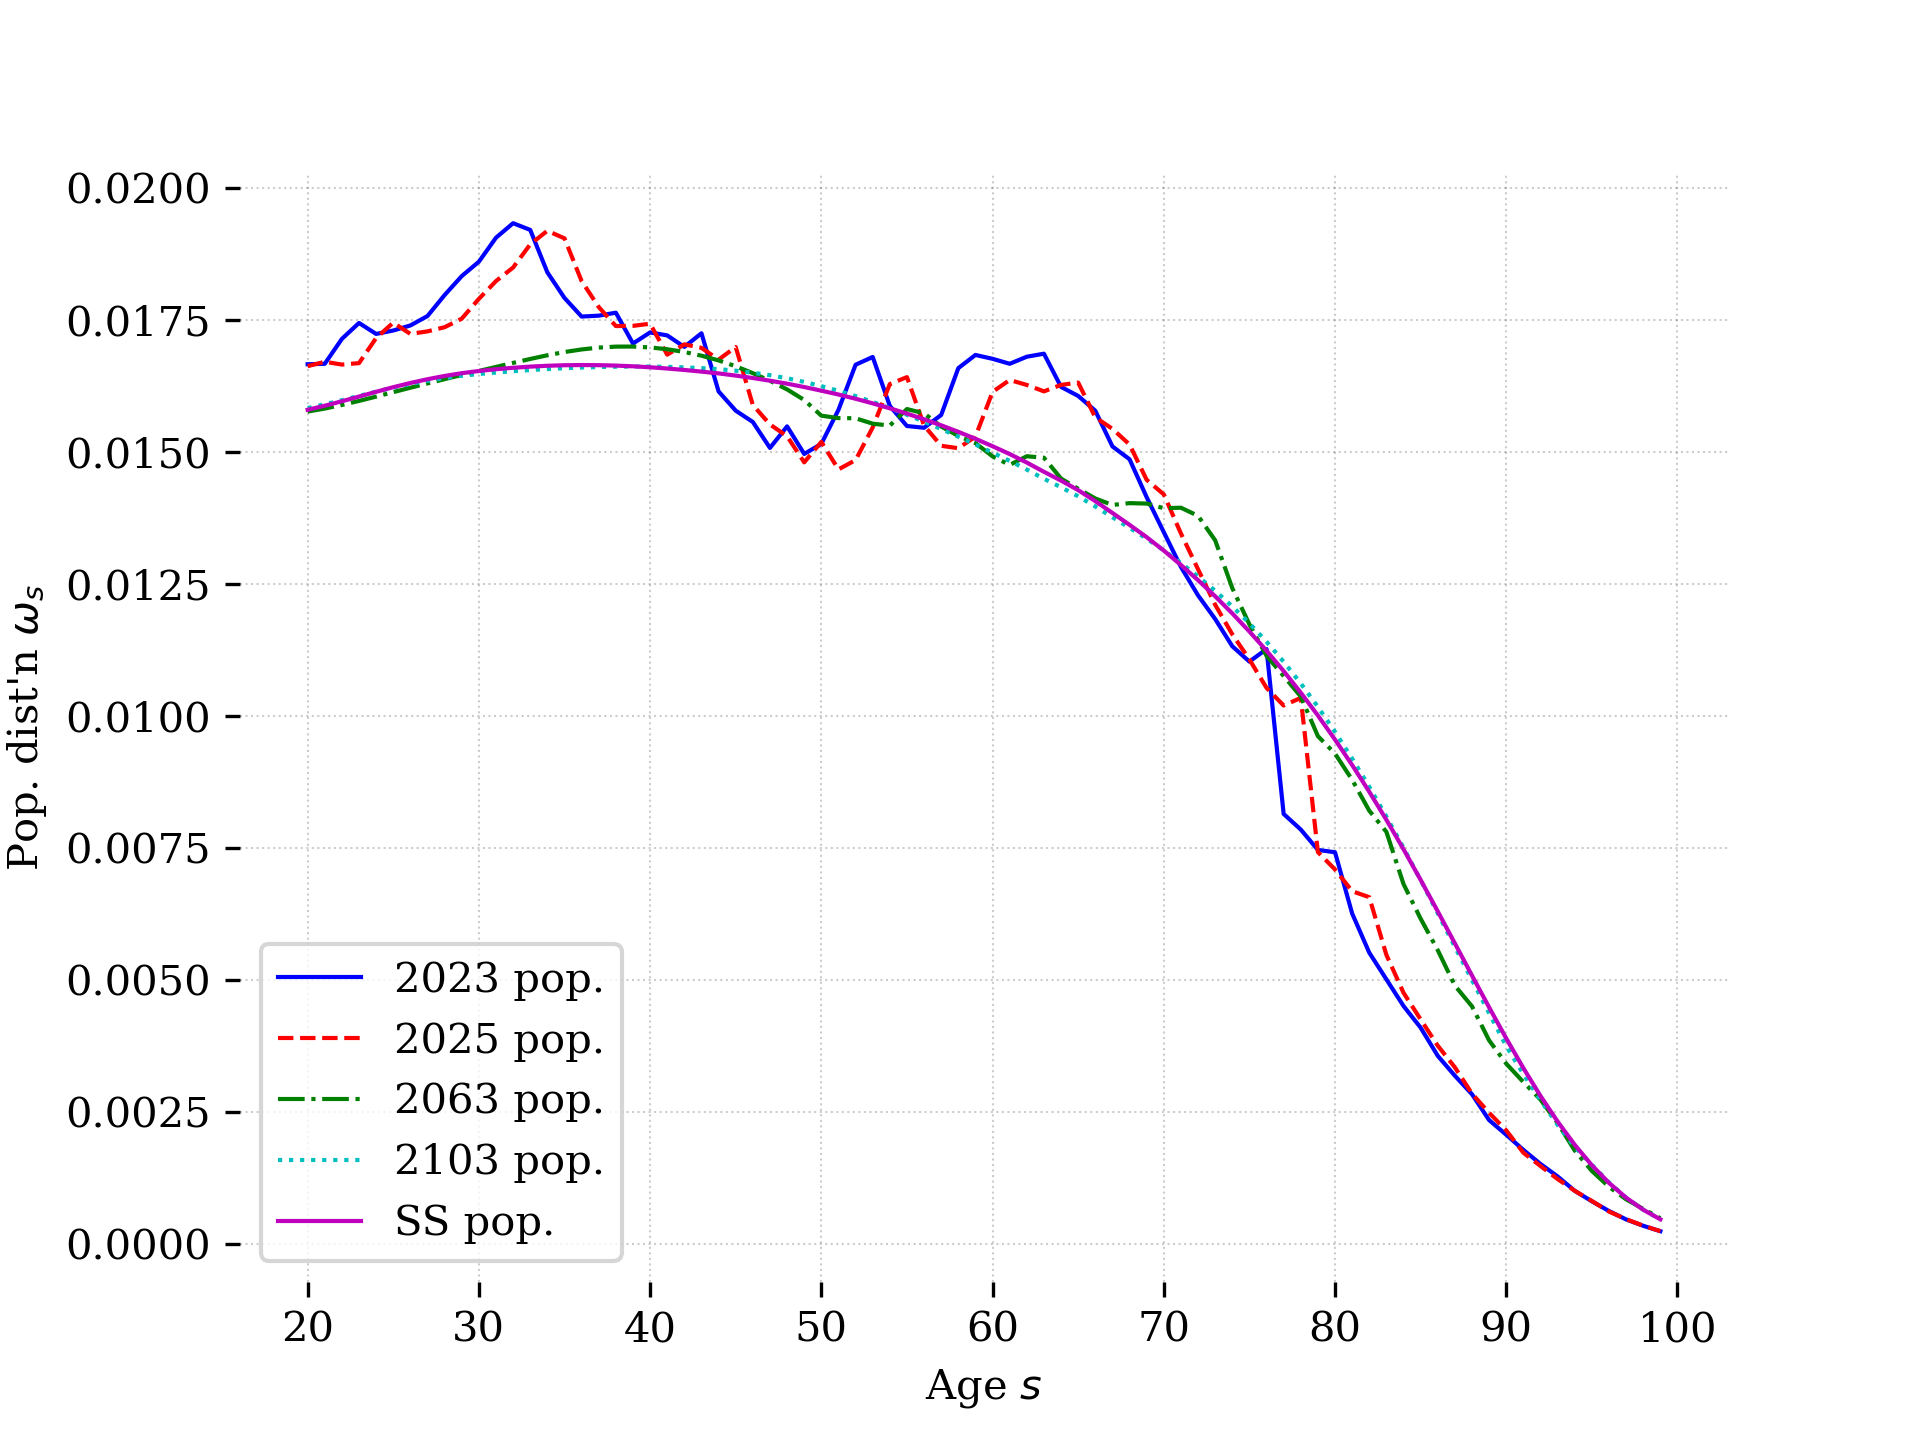
\includegraphics[height=0.8\textheight]{./images/USA_pop_distribution.png}
  \end{figure}
\end{frame}

\begin{frame}
  \frametitle{Compare to South Africa: Demographics, pop. distribution}
    \begin{figure}[htb]\centering
    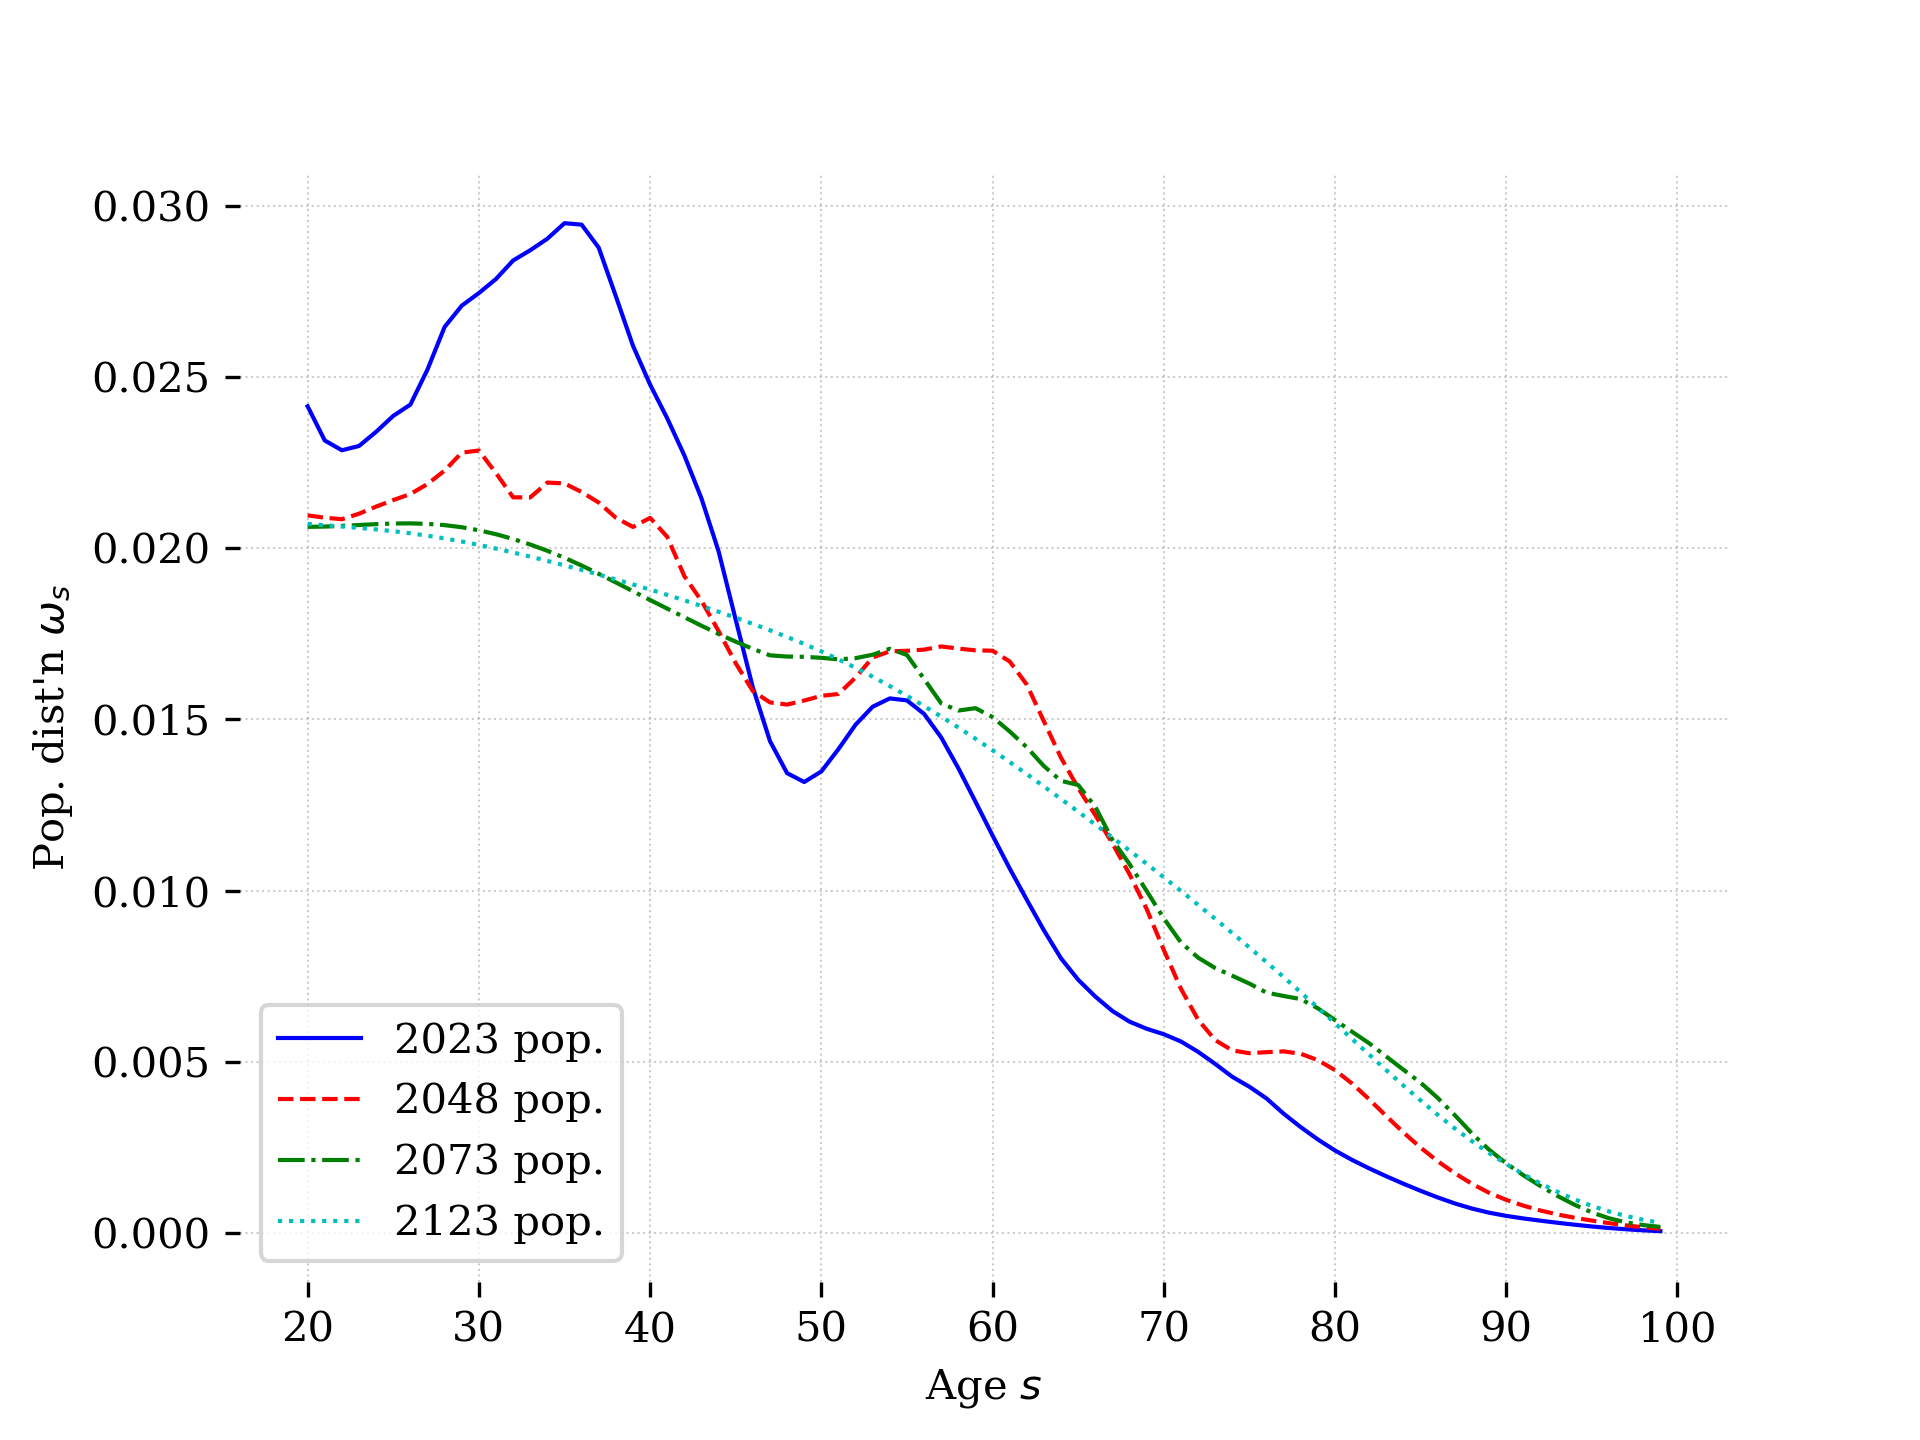
\includegraphics[height=0.8\textheight]{./images/ZAF_pop_distribution.png}
    \end{figure}
  \end{frame}

  \begin{frame}
\frametitle{Population Distribution Comparison}
 \begin{figure}[ht]
      \begin{minipage}[b]{0.35\linewidth}
          \centering
          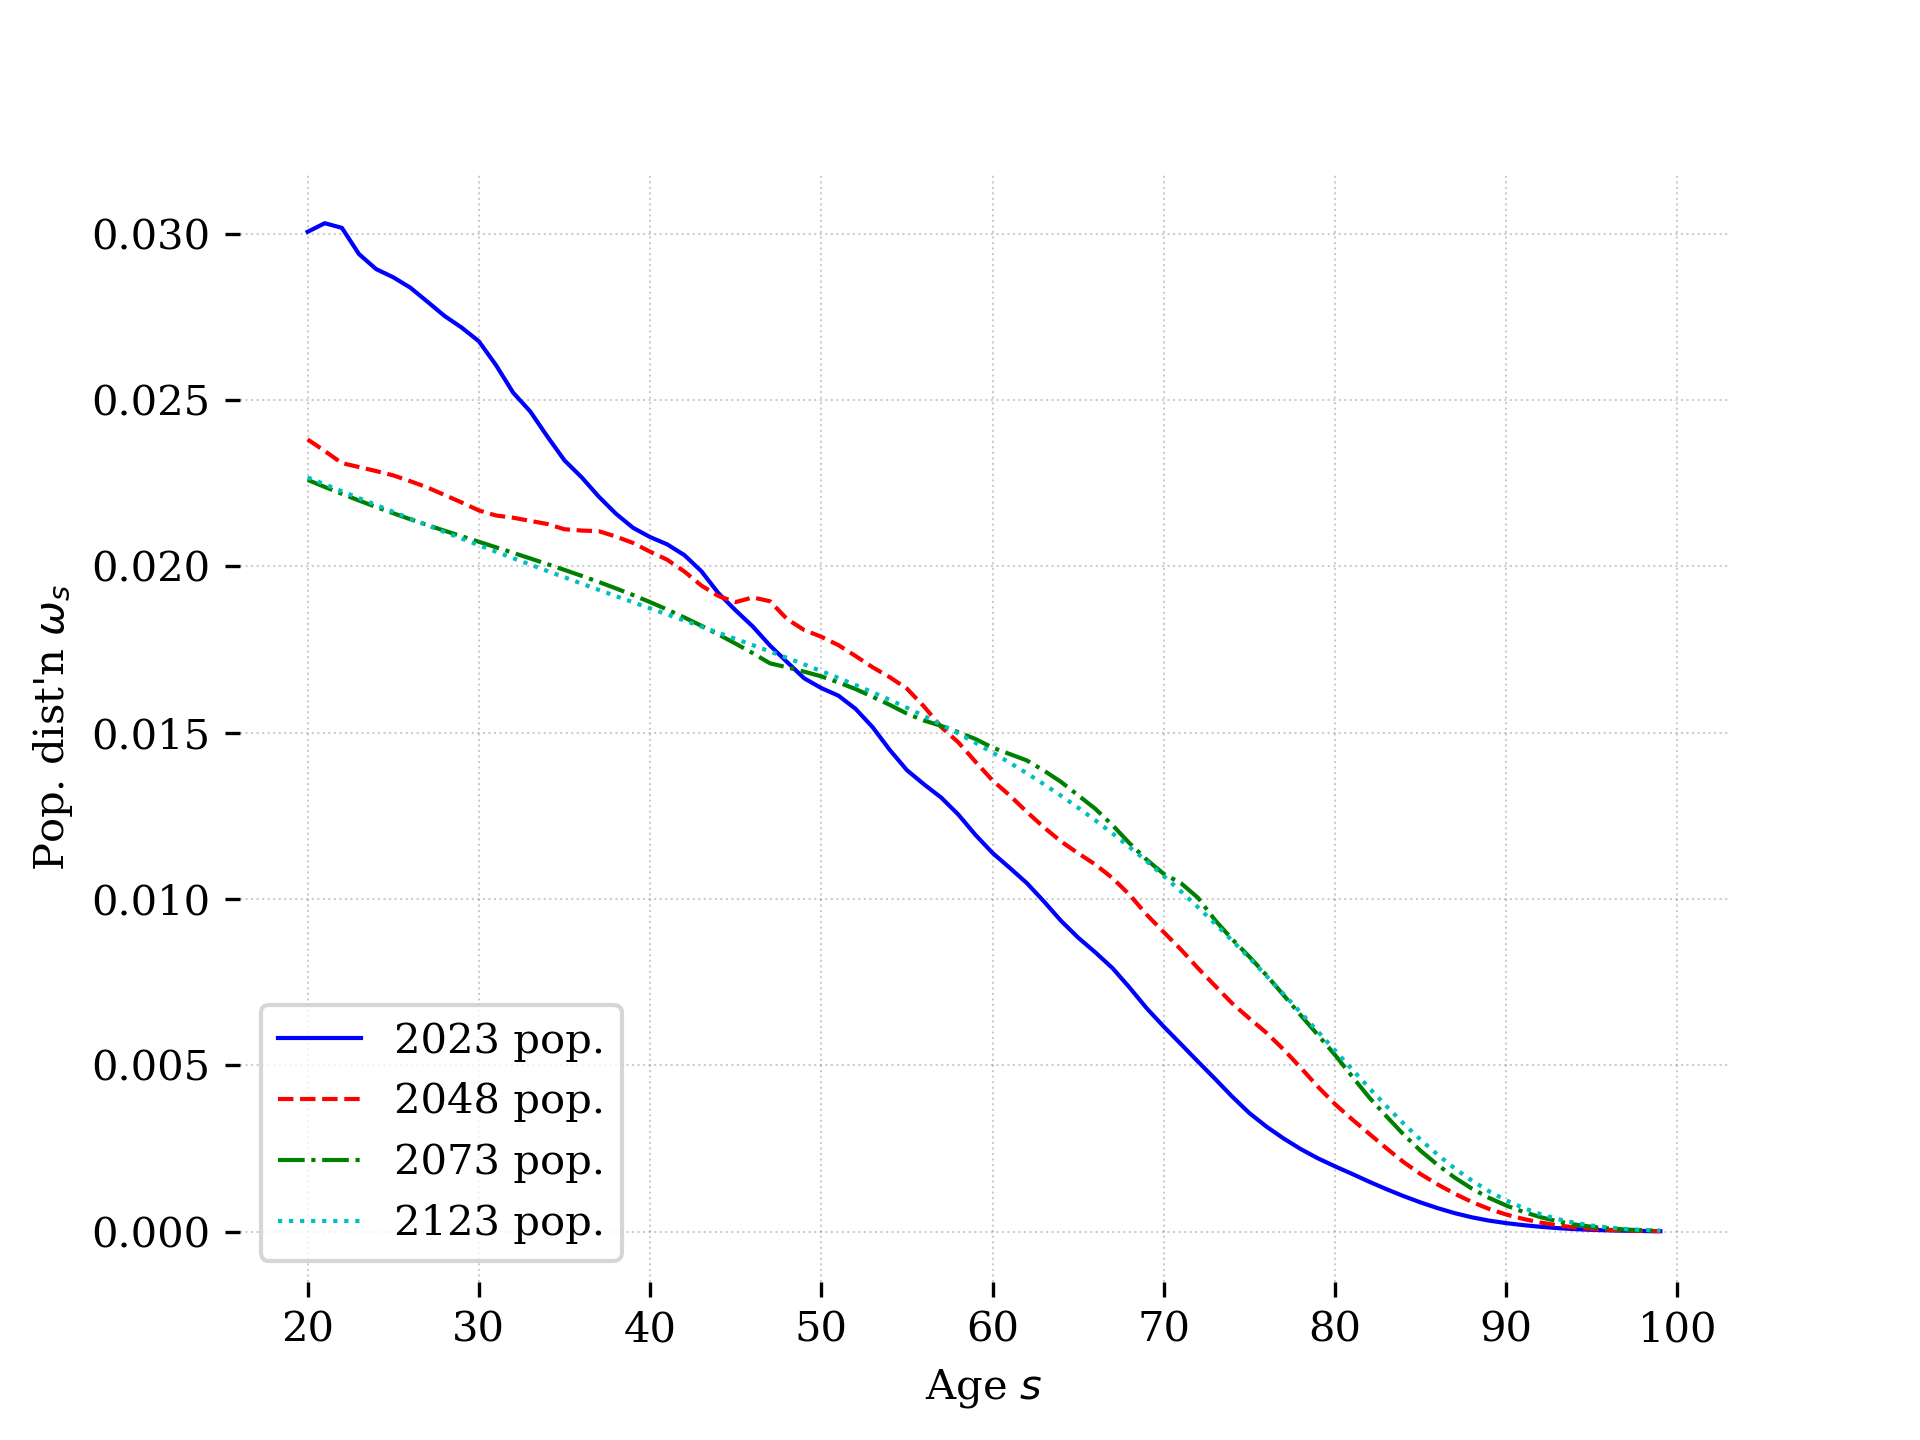
\includegraphics[width=\textwidth]{./images/pop_distribution.png}
          \caption{Philippines}
      \end{minipage}
      \hspace{0.5cm}
      \begin{minipage}[b]{0.35\linewidth}
          \centering
          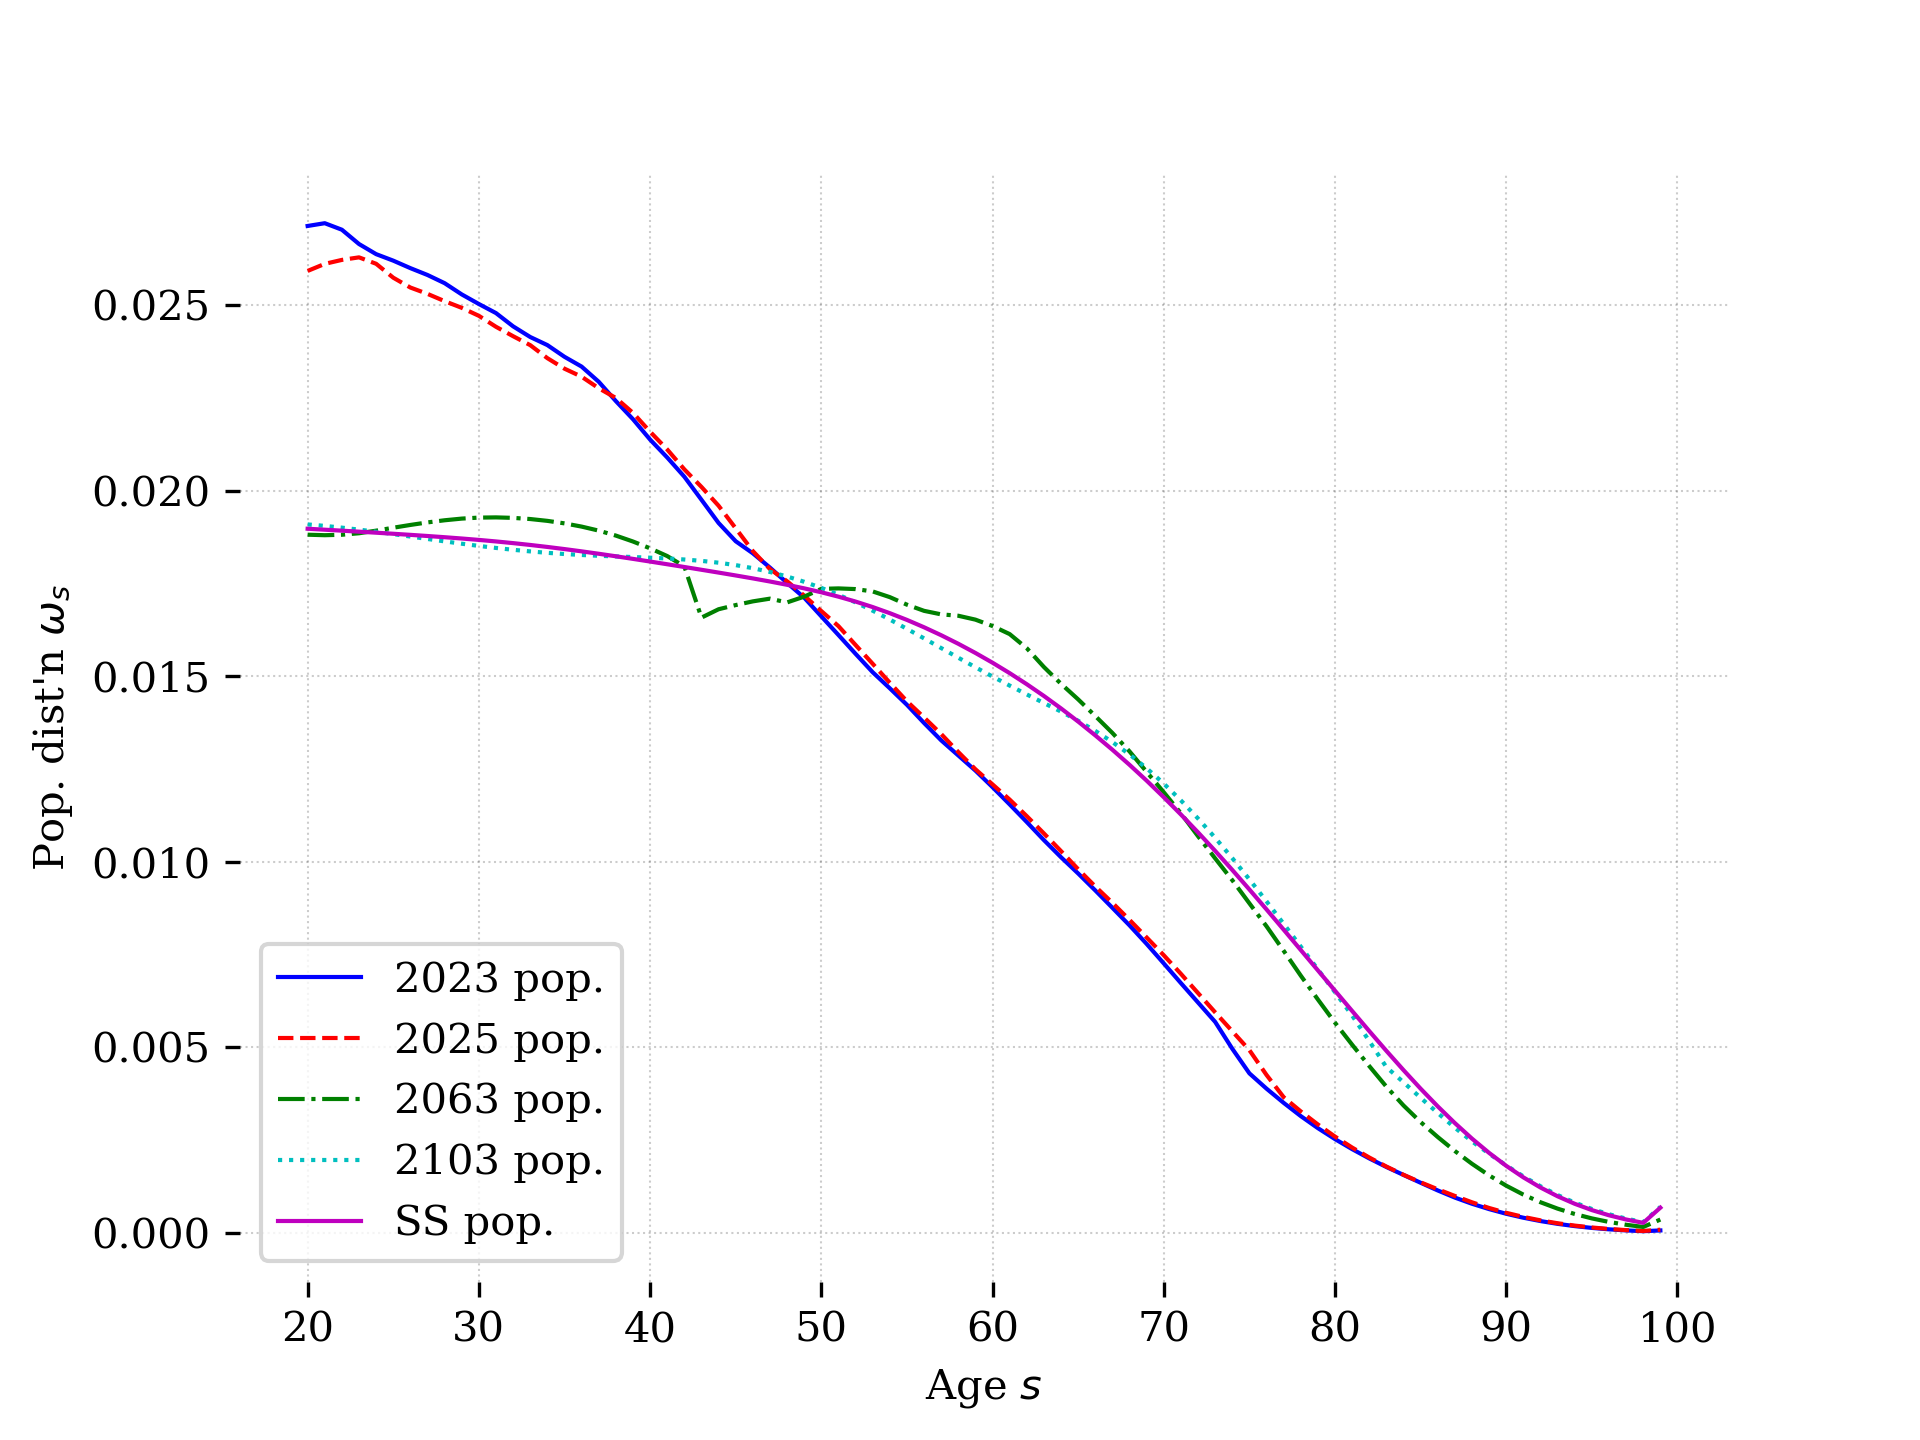
\includegraphics[width=\textwidth]{./images/IND_pop_distribution.png}
          \caption{India}
      \end{minipage}
      \begin{minipage}[b]{0.35\linewidth}
          \centering
          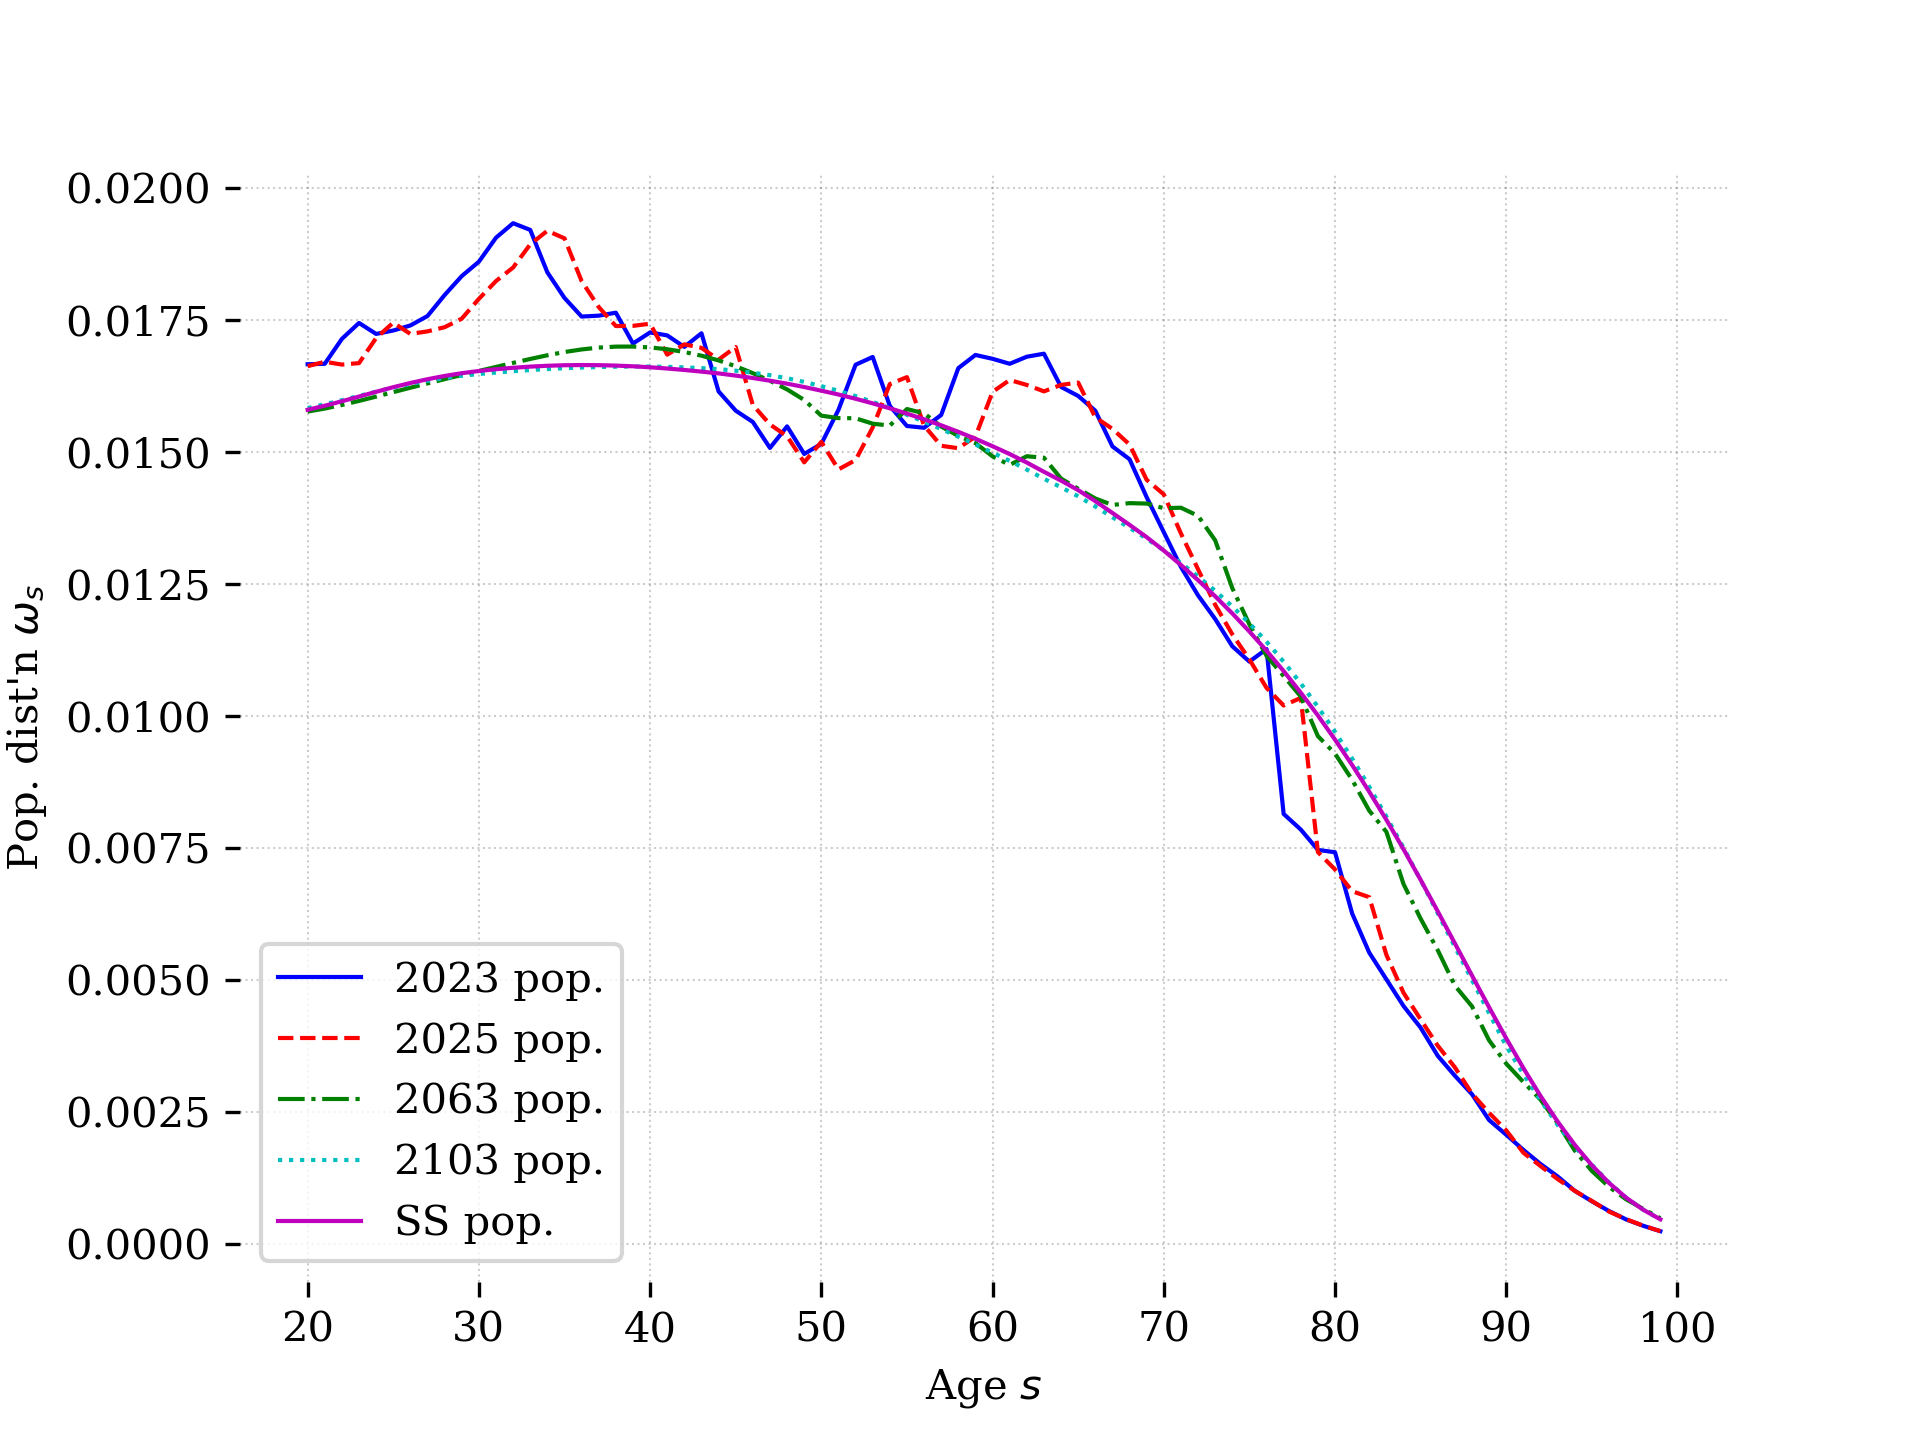
\includegraphics[width=\textwidth]{./images/USA_pop_distribution.png}
          \caption{United States}
      \end{minipage}
      \begin{minipage}[b]{0.35\linewidth}
        \centering
        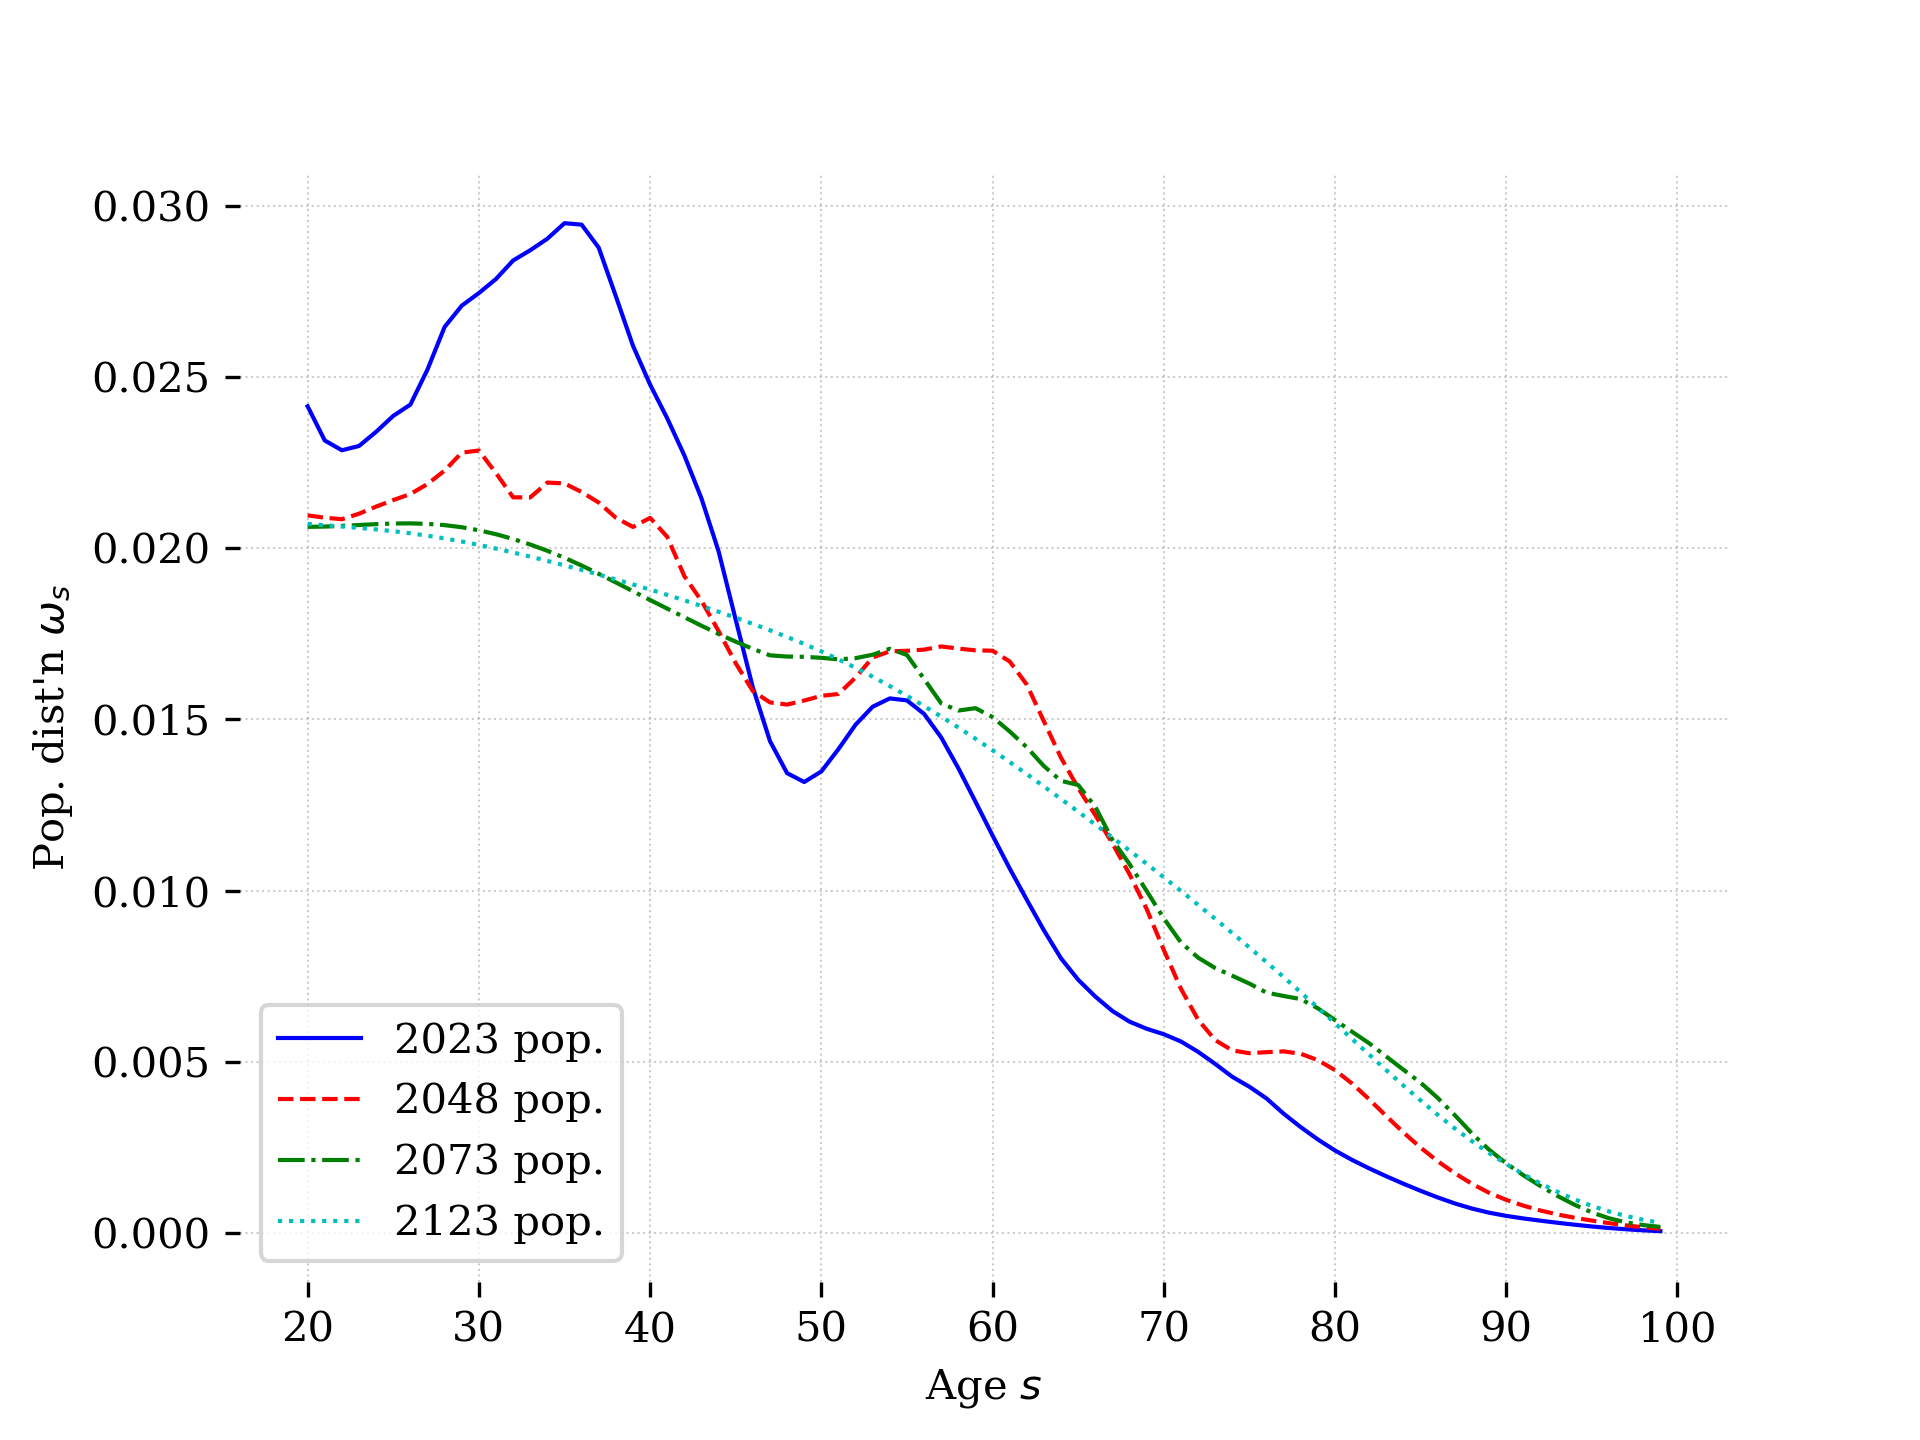
\includegraphics[width=\textwidth]{./images/ZAF_pop_distribution.png}
        \caption{South Africa}
    \end{minipage}
  \end{figure}
 \end{frame}

\begin{frame}
\frametitle{Demographics, pop. growth}
  \begin{figure}[htb]\centering
  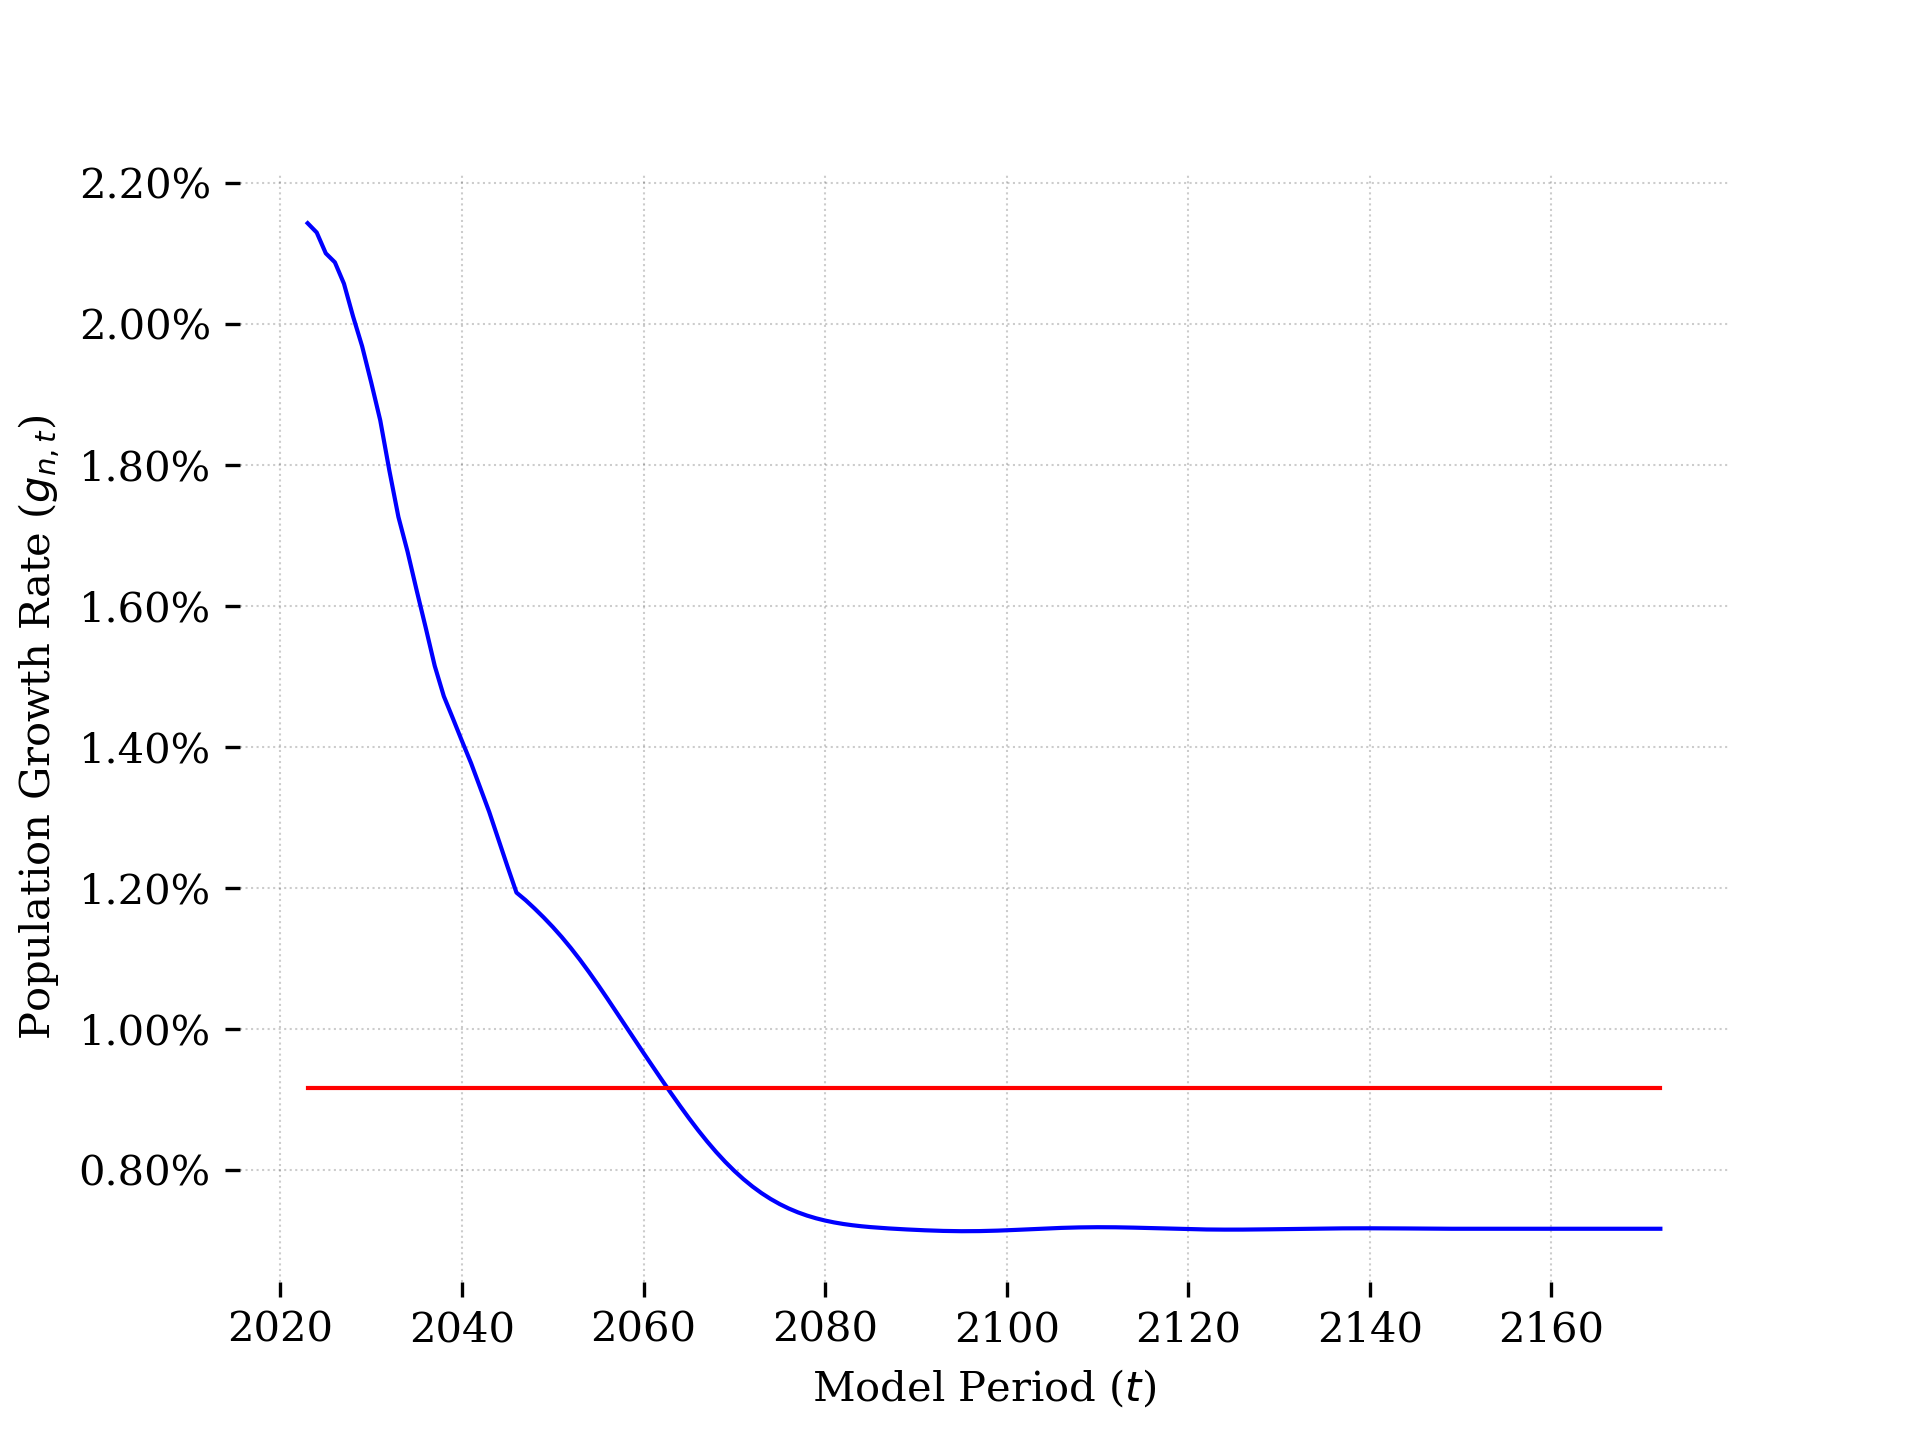
\includegraphics[height=0.8\textheight]{./images/population_growth_rates.png}
  \end{figure}
\end{frame}

\section{Earnings}
 \begin{frame}{Earnings Ability}
  \begin{itemize}
      \item Households are heterogeneous earnings ability/effective labor units
          \begin{itemize}
              \item There is a (endogenously determined) common wage rate per effective unit of labor, but households vary in the effective units of labor per unit of labor supply, giving rise to differences in hourly earnings

  \begin{equation*}
    c_{j,s,t} + b_{j,s+1,t+1} = (1 + r_{t})b_{j,s,t} + \textcolor{red}{w_t e_{j,s} n_{j,s,t}} + ...
  \end{equation*}

              \item Earnings ability varies across households and over the lifecycle within a household
          \end{itemize}
      \item There is no earnings risk: while earnings vary over the lifecycle, this process is completely deterministic
      \item Effective labor units are homogeneous from the point of view of firms
      \item No human capital accumulation decisions: earnings ability profiles are exogenous
  \end{itemize}
 \end{frame}

  \begin{frame}
\frametitle{Calibrating Lifetime Earnings Profiles}
  \begin{itemize}
      \item Ideally, one can estimate the lifetime earnings profiles from microdata that represents a long panel of households (see e.g., Fullerton and Rogers (1993) or DeBacker et al. (2016))
      \item However, these data are often hard to come by
      \item We've therefore devised a reasonable approximation that requires only minimal data:
          \begin{itemize}
              \item Begin with the earnings profiles for U.S. household estimated by DeBacker et al. (2016)
              \item Using single parameter function, adjust the shape of the profiles for each earnings group to match the gini coefficient in Philippines
          \end{itemize}
  \end{itemize}
\end{frame}

    \begin{frame}{Data: Labor Productivity Profiles}
      \begin{itemize}
        \item National Transfer Account data
        \begin{itemize}
          \item Distribution of income by age
        \end{itemize}
        \item \href{https://data.worldbank.org/indicator/SI.POV.GINI?locations=PH}{World Bank WDI}
          \begin{itemize}
            \item Overall inequality
          \end{itemize}
      \end{itemize}
    \end{frame}

\begin{frame}
\frametitle{OG-PHL Lifetime Earnings Profiles}
% Gini coefficient (income, 2005): USA: 41, PHL: 40.7
     \begin{figure}[ht]
      \begin{minipage}[b]{0.45\linewidth}
          \centering
          USA Gini = 41.0
          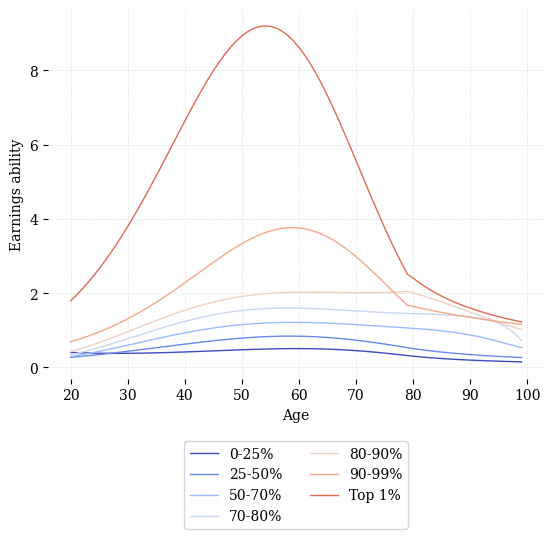
\includegraphics[width=0.85\textwidth]{./images/USA_ability_profiles.png}
          \caption{Earnings Profiles, USA}
          \label{fig:earnings_USA}
      \end{minipage}
      \hspace{0.5cm}
      \begin{minipage}[b]{0.45\linewidth}
          \centering
          PHL Gini = 40.7
          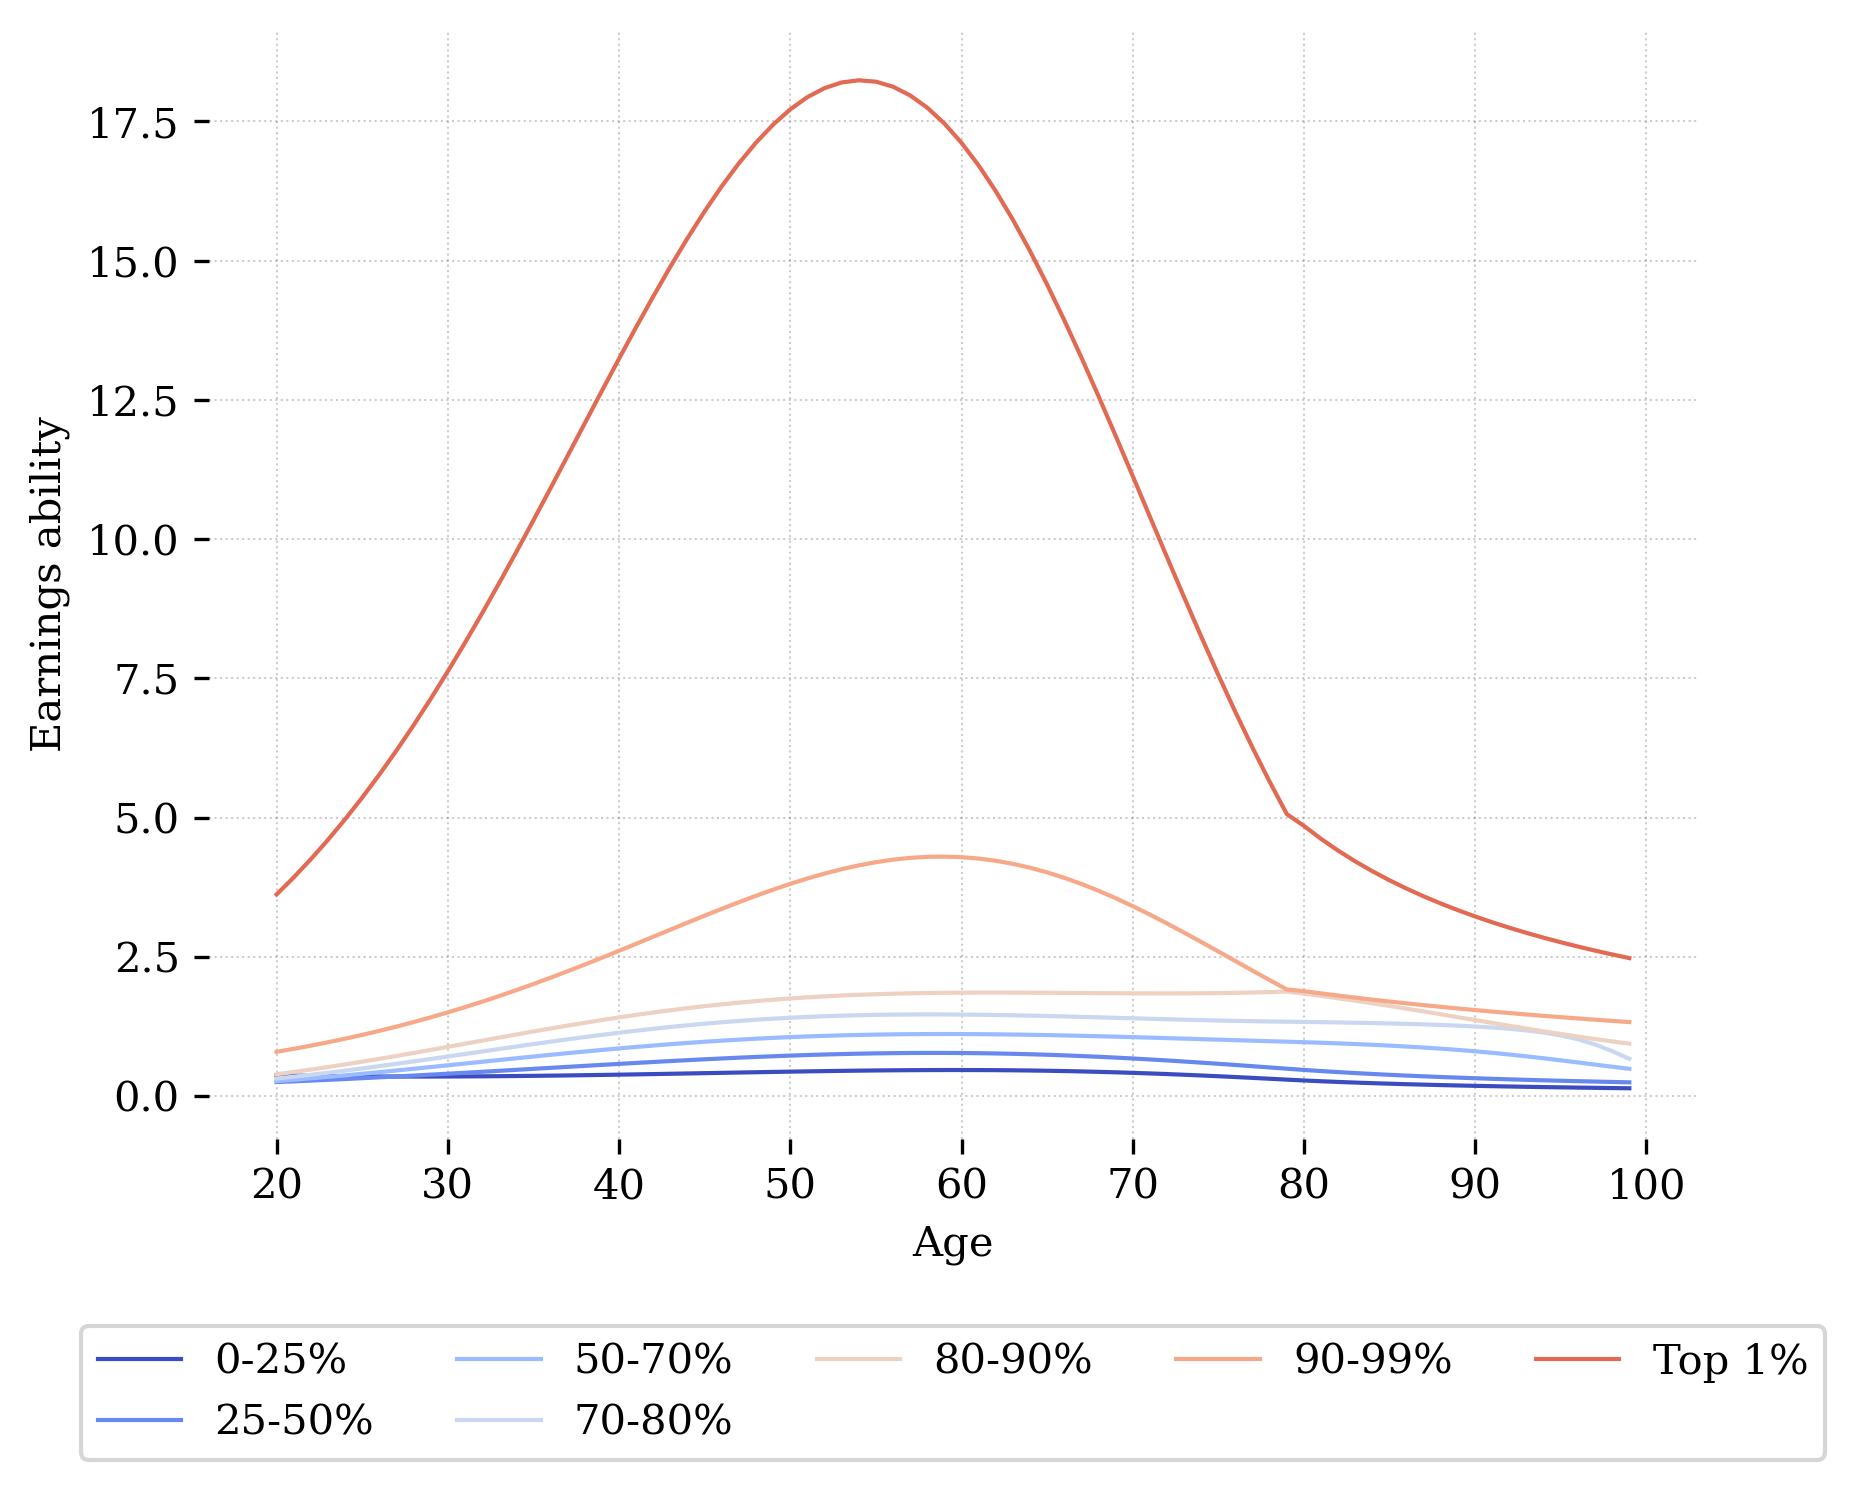
\includegraphics[width=\textwidth]{./images/PHL_ability_profiles.png}
          \caption{Earnings Profiles, PHL}
          \label{fig:earnings_PHL}
      \end{minipage}
  \end{figure}
\end{frame}

\section{Supply Side}
% \begin{frame}
%   \frametitle{Calibrating Firm Parameters}
%   \begin{itemize}
%     \item Marcelo was able to use the PHL national accounts data
%       \begin{itemize}
%           % \item Output, labor, capital by industry $\implies$ industry TFP
%           \item Labor's share of output by industry
%       \end{itemize}
%   \end{itemize}
%   \small
%   \begin{table}[]
% \begin{tabular}{lrrc}
% \hline
% \hline
%                  & \multicolumn{1}{c}{TFP} & \multicolumn{1}{c}{TFP} & \multicolumn{1}{c}{Capital Share} \\
%         Production Sector                & \multicolumn{1}{c}{$(GVA/F(K,L))$} & \multicolumn{1}{c}{(normalized)}& \multicolumn{1}{c}{Income} \\
%     \hline
% Primary & 396.80   &   0.11  & 0.67   \\
% Secondary (ex energy) &  3474.10  & 1.00 & 0.50   \\
% Tertiary & 6604.17   &  1.90 & 0.45  \\
% Energy        & 551.63   &  0.16  & 0.53  \\ \hline
% \end{tabular}
% \end{table}
% \end{frame}

\begin{frame}
  \frametitle{Firm Production Technology}
  \begin{itemize}
      \item Use national accounts data to calibrate the firm production function:

      \begin{equation*}
        \begin{split}
          Y_{m,t} &= F(K_{m,t}, K_{g,m,t}, L_{m,t}) \\
          &\equiv Z_{m,t}\biggl[(\textcolor{red}{\gamma_m})^\frac{1}{\varepsilon_m}(K_{m,t})^\frac{\varepsilon_m-1}{\varepsilon_m} + (\gamma_{g,m})^\frac{1}{\varepsilon_m}(K_{g,m,t})^\frac{\varepsilon_m-1}{\varepsilon_m} + \\
          &\quad\quad\quad\quad\quad(1-\textcolor{red}{\gamma_m}-\gamma_{g,m})^\frac{1}{\varepsilon_m}(e^{g_y t}L_{m,t})^\frac{\varepsilon_m-1}{\varepsilon_m}\biggr]^\frac{\varepsilon_m}{\varepsilon_m-1} \quad\forall m,t
        \end{split}
      \end{equation*}
      \item Capital share of output: $\gamma_m = 0.588$

      \item Set $\varepsilon_m = 1.0$ for all sectors (Cobb-Douglas production)
  \end{itemize}
\end{frame}


\begin{frame}{Data: Firm Production}
  \begin{itemize}
    \item UN \href{https://ilostat.ilo.org}{ILOSTAT} data
      \begin{itemize}
        \item Capital's share of income (overall)
      \end{itemize}
    \item \href{https://databank.worldbank.org/source/world-development-indicators}{World Bank Development Indicators}
      \begin{itemize}
        \item Long run growth rate in real GDP per capita
      \end{itemize}
  \end{itemize}
  \end{frame}

\begin{frame}
  \frametitle{Mapping Production Goods to Consumption Goods}
  \begin{itemize}
    \item Model households consume differentiated goods:
      \begin{equation*}
        c_{j,s,t} \equiv \prod_{i=1}^I \left(c_{i,j,s,t} - c_{min,i}\right)^{\textcolor{red}{\alpha_i}} \quad\forall j,s,t \quad\text{with}\quad \sum_{i=1}^I\alpha_i=1
      \end{equation*}

      \item Consumption goods are composites of production goods, determined via fixed proportions:

      \begin{equation*}
        \tilde{p}_{i,t} = \sum_{m=1}^M \textcolor{red}{\pi_{i,m}}\tilde{p}_{m,t} \quad\forall i,t
      \end{equation*}
    \end{itemize}
  \end{frame}

  \begin{frame}
    \frametitle{Mapping Production Goods to Consumption Goods}
    \begin{itemize}
      \item This leaves two parameter objects to calibrate:
          \begin{enumerate}
              \item Household preferences (expenditure shares) over the differentiated production goods, $\alpha_i$
              \item A matrix representing the shares of each output good in the composition of each consumption good, $\Pi$
          \end{enumerate}
  \end{itemize}
\end{frame}


\begin{frame}
  \frametitle{Data Mapping Production Goods to Consumption Goods}
  \begin{itemize}
      \item Data for these are contained in standard ``social accounting matrices'' used in CGE modeling
      \item These are readily available for most countries from \href{https://www.gtap.agecon.purdue.edu}{GTAP} or other sources
      \item For the PHL calibration, we use \href{https://dataverse.harvard.edu/file.xhtml?fileId=5617690&version=1.0}{data from the International Food Policy Research Institute}
  \end{itemize}
\end{frame}

\begin{frame}
  \frametitle{Calibration of IO Matrix and Consumption Shares}
  \footnotesize
  \begin{table}
  \caption{Consumption-Production Bridge Matrix}
  \begin{tabular}{lrrrrrrr}
    \hline
    \hline
     & Agr & Mining & Util & Cons. & Trade \& & Serv & Manu \\
     & \& Fish &  & &  & Trans & &  \\
    \hline
    Food & 0.120 & 0.000 & 0.000 & 0.002 & 0.047 & 0.153 & 0.679 \\
    Energy \& & 0.005 & 0.009 & 0.113 & 0.057 & 0.066 & 0.206 & 0.543 \\
    \ \ Extraction &  &  &  &  &  &  &  \\
    Non-durables & 0.023 & 0.013 & 0.012 & 0.315 & 0.130 & 0.183 & 0.323 \\
    Durables & 0.004 & 0.005 & 0.013 & 0.048 & 0.067 & 0.120 & 0.743 \\
    Services & 0.035 & 0.004 & 0.004 & 0.045 & 0.206 & 0.520 & 0.185 \\
    \hline
    \end{tabular}
\end{table}

  \begin{table}
  \caption{Consumption Expenditure Shares}
  \begin{tabular}{lrrrr}
\hline
\hline
Food & Energy & Non-durables & Durables & Services \\
Food & \& Extraction & &  & \\
\hline
0.357 & 0.014 & 0.021 & 0.103 & 0.505 \\
\hline
\end{tabular}
\end{table}

\end{frame}

\section{Macro}
\begin{frame}{Macroeconomic parameters:}
\begin{itemize}
  \item Long run growth rate, $g_y= 3.6\%$ (growth in GDP per capita from 2000 to 2019)
  \item Initial period debt-to-GDP ratio, 60\%
  \item Open economy parameters:
    \begin{itemize}
      \item Initial percentage of debt held by foreigners, 14.6\%
      \item Percentage of newly issued debt purchased by foreigners, 14.6\%
      \item Openness of capital flow (0 to 1 scale), 0.9
    \end{itemize}
  \item Government spending:
    \begin{itemize}
      \item Non-pension transfers to GDP, 9.7\%
      \item Government consumption expenditures to GDP, 14.2\%
    \end{itemize}
\end{itemize}
\end{frame}

\begin{frame}{Macro data}
  \begin{itemize}
    \item \href{https://www.imf.org/external/datamapper/profile/PH}{IMF} data
      \begin{itemize}
        \item Government spending
      \end{itemize}
    \item \href{https://databank.worldbank.org/source/world-development-indicators}{World Bank Development Indicators}
      \begin{itemize}
        \item Foreign purchases of new debt issues
        \item Long run growth rate in real GDP per capita
        \item Government consumption expenditure
      \end{itemize}
  \end{itemize}
  \end{frame}

\section{Future}

\begin{frame}{To come:}
\begin{itemize}
  \item More detail with tax and benefit system
  \item Match distribution of wealth
  \item Calibrate labor supply to match rates in Philippines
    \begin{itemize}
      \item Note: model is of cohorts of agents, so unemployment not directly modeled, but we can get at it through, e.g., low labor supply of the young
    \end{itemize}
\end{itemize}
\end{frame}

\begin{frame}{Household Survey Data}
    \begin{itemize}
      \item Would like this to include:
        \begin{itemize}
          \item Labor supply
          \item Net wealth
          \item Income taxes paid
          \item Informal economic activity
        \end{itemize}
      \item Which \href{https://psada.psa.gov.ph/catalog/Household-based_Surveys/about}{household survey} from the Philippines Statistical Authority would best to use?  Or something else?
    \end{itemize}
  \end{frame}

    \begin{frame}{Household Survey Data}
    \begin{itemize}
      \item What these can enable:
        \begin{itemize}
          \item Calibrate disutility of labor supply to match hours worked by age
          \item Calibrate rate of time preference/bequest motives to match distribution of wealth
          \item Estimation of tax functions that allow for tax progressivity
          \item Calibration of informal production/consumption
          \item Distribution of government transfers
          \item Distribution of bequests
        \end{itemize}
    \end{itemize}
  \end{frame}

\begin{frame}
  \frametitle{Matching labor supply, US Example}
    \begin{figure}[htb]\centering
    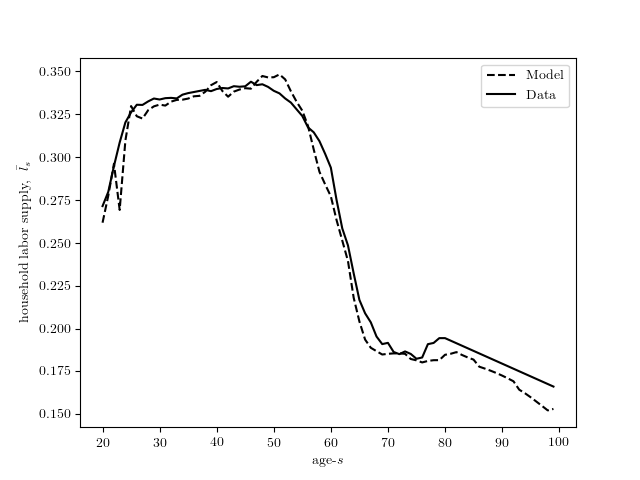
\includegraphics[height=0.8\textheight]{./images/labor_dist_comparison.png}
    \end{figure}
  \end{frame}



    \begin{frame}
      \frametitle{Tax Functions, US Example}
        \begin{figure}[htb]\centering
        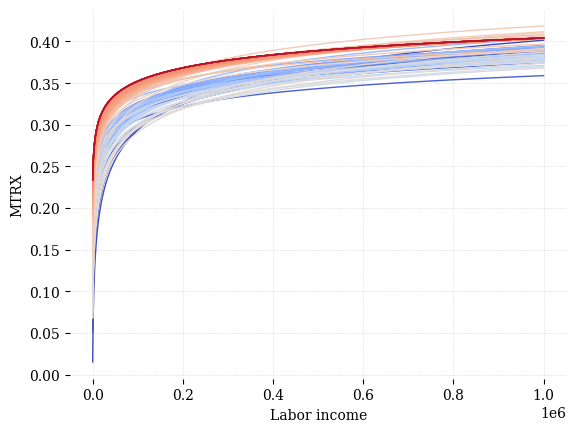
\includegraphics[height=0.8\textheight]{./images/HSV_PUF_mtrx.png}
        \end{figure}
      \end{frame}


  \begin{frame}{National accounts data by sector}
    \begin{itemize}
      \item Could also benefit from some more detail:
        \begin{itemize}
          \item Sector specific TFP
          \item Sector specific capital shares
          \item Factor prices by industry $\implies$ ability to estimate elasticity of substitution
          \item Structure of production in the informal sector
          \item Small vs large firms
          \item What is the role of public infrastructure in private production?
        \end{itemize}
    \end{itemize}
  \end{frame}

  \begin{frame}{Other?}
    \begin{itemize}
      \item Policy parameters:
        \begin{itemize}
          \item Pension benefits
          \item Infrastructure spending (as fraction of GDP)
          \item Identifying transitory policies and accounting for them in the calibration
        \end{itemize}
      \item Applied micro studies in Philippines to estimate basic household preference parameters:
        \begin{itemize}
          \item Intertemporal elasticity of substitution, $\sigma$
          \item Frisch elasticity of labor supply, $\theta$
          \item Rate of time preference, $\beta$
          \item Stone-Geary preferences (``subsistence'' consumption by good, $c_{min, i}$, which leads to non-homothetic preferences)
        \end{itemize}
    \end{itemize}
    \end{frame}


\end{document}
